% !TeX program = xelatex
\documentclass[acmtog,anonymous,review]{acmart}

\usepackage{graphicx}
\usepackage{amsmath}
\usepackage{booktabs}
\usepackage{xcolor}
\usepackage{algorithm}
\usepackage{algpseudocode}

\settopmatter{printacmref=true}
\citestyle{acmauthoryear}
\addtolength{\textfloatsep}{8pt}
\addtolength{\dbltextfloatsep}{8pt}
\addtolength{\floatsep}{4pt}
\addtolength{\dblfloatsep}{4pt}
\acmSubmissionID{2781}
\renewcommand\footnotetextcopyrightpermission[1]{}

\title{Projection-Stabilized Execution for Recursive Sparse 3D Latents}

\author{Anonymous Author(s)}
\affiliation{%
  \institution{Anonymous Institution}
  \city{}
  \country{}
}
\email{}

\begin{document}

\begin{abstract}
We study finite-depth recursive 3D asset generation, where authored rules expand branches, frontiers, copied motifs, and local regions that must remain readable by later steps, while sparse latent 3D generators provide native support, token features, codec operations, and learned local priors. Projection-Stabilized Recursive Sparse-Latent Execution (PS-RSLE) adds the execution layer that turns decoded geometry into reusable executable state by wrapping a frozen sparse latent generator with active handles for local frames, ownership, frontiers, attachments, and motifs. Rules emit typed proposals, controlled sparse-latent sampling realizes admitted local surface and feature edits, and projection with codec re-entry commits root-attached or connector-certified support before the next rule fires. In this frozen-generator instantiation, the executor stabilizes per-depth executable state, spans branching, frontier-growth, and transform-copy assets, maintains high largest-component ratios under the reported surface proxy, and improves welded mesh fragmentation and rendered local readability.
\end{abstract}

\begin{CCSXML}
<ccs2012>
 <concept>
  <concept_id>10010147.10010371.10010396.10010397</concept_id>
  <concept_desc>Computing methodologies~Shape modeling</concept_desc>
  <concept_significance>500</concept_significance>
 </concept>
 <concept>
  <concept_id>10010147.10010371.10010352.10010236</concept_id>
  <concept_desc>Computing methodologies~Mesh geometry models</concept_desc>
  <concept_significance>500</concept_significance>
 </concept>
 <concept>
  <concept_id>10010147.10010371.10010396</concept_id>
  <concept_desc>Computing methodologies~Computer graphics</concept_desc>
  <concept_significance>300</concept_significance>
 </concept>
</ccs2012>
\end{CCSXML}

\ccsdesc[500]{Computing methodologies~Shape modeling}
\ccsdesc[500]{Computing methodologies~Mesh geometry models}
\ccsdesc[300]{Computing methodologies~Computer graphics}

\keywords{recursive 3D generation, procedural modeling, Sparse Latent 3D Generators, projection, executable state}

\begin{teaserfigure}
  \centering
  \includegraphics[width=\textwidth]{figures/personal/teaser.pdf}
  \Description{Compact front-view render strip of five recursive 3D assets: bismuth crystal, pyrite lattice, coral, tree-root foliage, and vine-root foliage.}
  \caption{Recursive sparse-latent outputs spanning transform-copy crystal and lattice assets, frontier-style coral growth, and branching root or vine structures.}
  \label{fig:teaser}
\end{teaserfigure}

\maketitle

\section{Introduction}

Recursive 3D asset generation targets structured objects whose form emerges through repeated local expansion. We study finite-depth, user-controlled programs for branching vegetation, accretive aggregates, crystals, lattices, and repeated motifs, patterns common in natural structures (Fig.~\ref{fig:natural-recursive-structures}) and procedural pipelines~\cite{shaker2016pcgbook,smelik2014survey,parish2001proceduralcities,wonka2003instantarchitecture,mueller2006procedural,prusinkiewicz1990abop,runions2007spacecolonization,hutchinson1981fractals,barnsley1988fractalsEverywhere,witten1981dla,sander2000dlaReview}.

\begin{figure}[t]
  \centering
  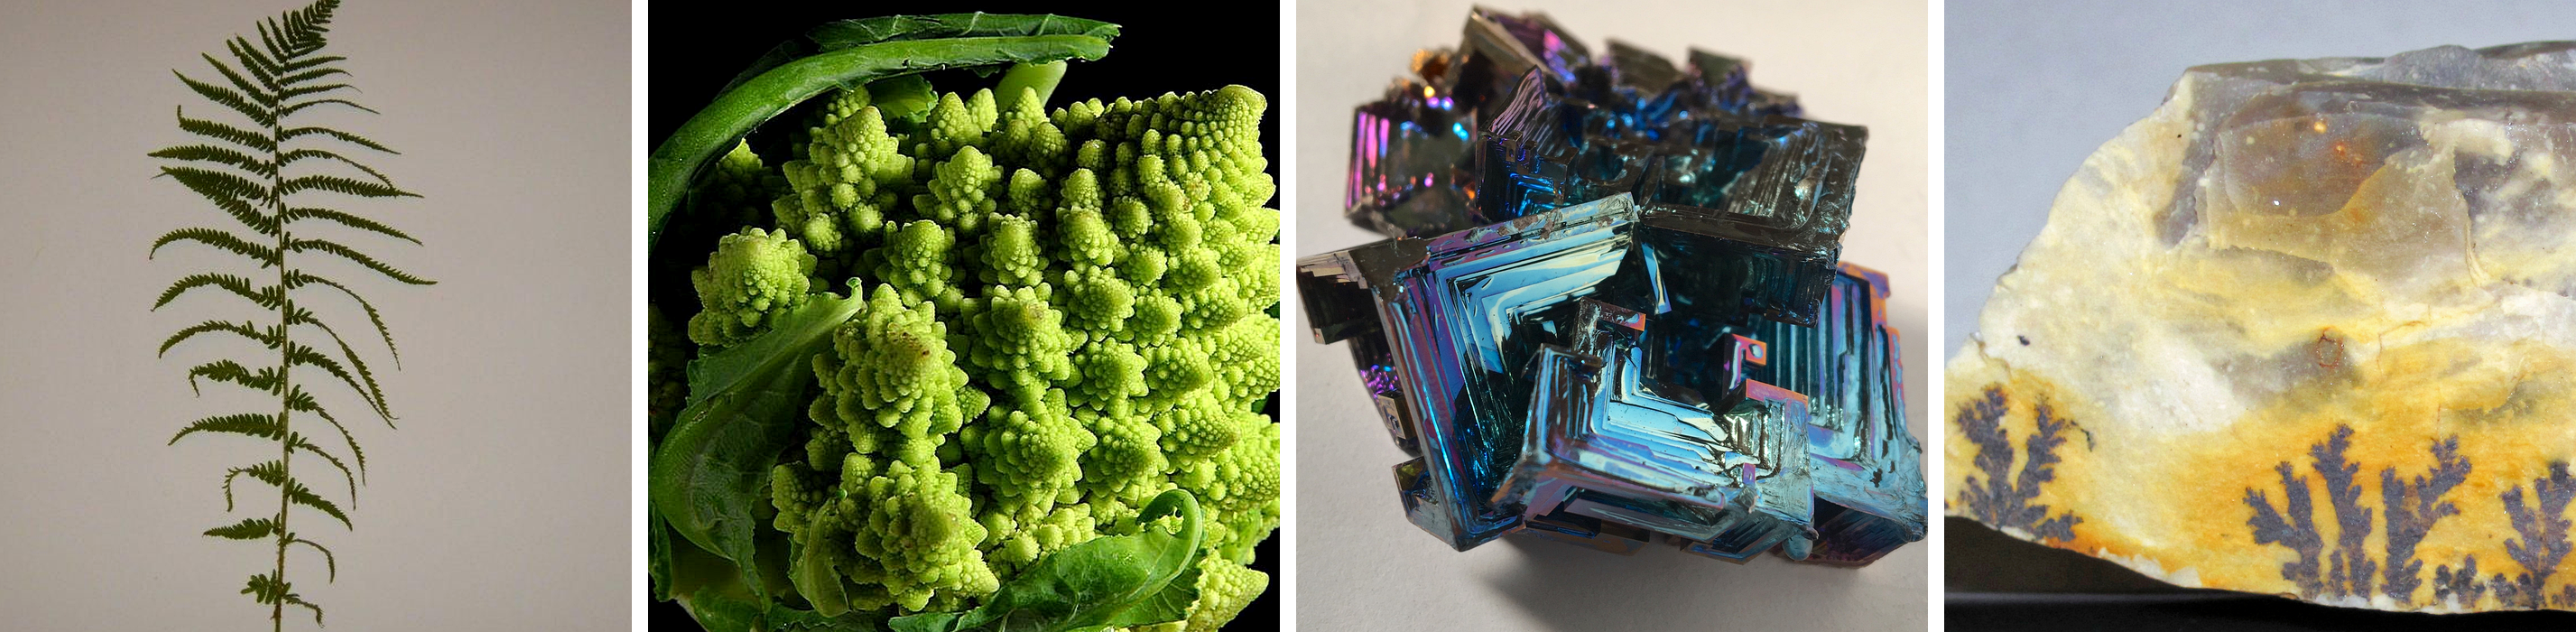
\includegraphics[width=\columnwidth]{figures/natural_recursive_structures_fourpanel.png}
  \Description{Four natural reference photographs showing recursive or self-similar structures: curled fern fronds, root-bound spider plant roots, a bismuth crystal, and manganese oxide dendrites on flint.}
  \caption{Natural recursive structures include repeated curled fronds, branching roots, stepped crystals, and dendritic accretion.}
  \label{fig:natural-recursive-structures}
\end{figure}

Recursive generation is an execution problem: local decisions build a tree, root network, coral aggregate, lattice motif, or repeated ornament, and each committed branch, frontier, motif, or edit region can become input to later decisions. The core requirement is executable state: intermediate geometry must remain editable, addressable, attached, and iterable across depth.

Classical procedural systems provide the structural side of this requirement, maintaining explicit symbols, tips, frontiers, transforms, or parts~\cite{lindenmayer1968lsystemsI,prusinkiewicz1990abop,hutchinson1981fractals,barnsley1988fractalsEverywhere,runions2007spacecolonization,witten1981dla,sander2000dlaReview,stiny1972shapegrammars,mueller2006procedural,smelik2014survey}. Sparse latent 3D generators provide complementary realization strength through token support, latent features, codec operations, and local sampling paths~\cite{trellis2025,trellis2project}.

The proposed executor combines these strengths in a single executable state: generator-native sparse latent tokens plus rule-readable active handles for local frames, ownership, frontiers, attachments, and motifs. Typed rules propose local sparse edits; controlled sparse-latent sampling realizes admitted proposals; projection and codec re-entry commit root-attached or connector-certified support into the next active state. The loop makes admissibility a per-depth execution invariant.

We instantiate the executor on a frozen sparse latent generator and evaluate branching, frontier-growth, and transform-copy assets. The experiments show that per-depth projection stabilizes executable state, that sparse-latent execution gives stronger recursive connectivity than one-shot or copy-based generator controls, and that our method maintains high surface largest-component ratios while reducing welded mesh fragmentation and improving rendered local readability.

\paragraph{Contributions.}
This paper makes the following contributions:
\begin{itemize}
  \item We formulate finite-depth recursive 3D asset generation as execution over a generator-coupled program state that combines native sparse latent support and features with rule-readable active handles.
  \item We define typed active-handle proposals and a per-depth state-stabilization loop: controlled sparse-latent sampling realizes local surface and feature edits, while admissibility projection and codec re-entry commit root-attached or connector-certified support before the next rule fires.
  \item We show that projection-stabilized sparse-latent execution supports branching, frontier-growth, and transform-copy assets while preserving reusable state across depth, improving connectivity and fragmentation against generator-space and mesh-space controls, and adding learned surface detail to classical procedural structures.
\end{itemize}

\section{Related Work}

\subsection{Procedural Recursive Modeling}

Procedural modeling provides explicit recursive state through L-systems, iterated function systems, space-colonization, diffusion-limited aggregation, and shape grammars~\cite{lindenmayer1968lsystemsI,prusinkiewicz1990abop,hutchinson1981fractals,barnsley1988fractalsEverywhere,runions2007spacecolonization,witten1981dla,sander2000dlaReview,stiny1972shapegrammars,mueller2006procedural,smelik2014survey}. Guided, inverse, and example-based variants reduce authoring effort~\cite{benes2011guidedprocedural,stava2010inverseprocedural,talton2011metropolisprocedural,ritchie2015controllingprocedural,nishida2016sketchingprocedural,ritchie2018exampleprocedural}. Our method keeps explicit symbol, frontier, and transform contracts while coupling rule proposals to a sparse-latent realization substrate.

\begin{figure}[t]
  \centering
  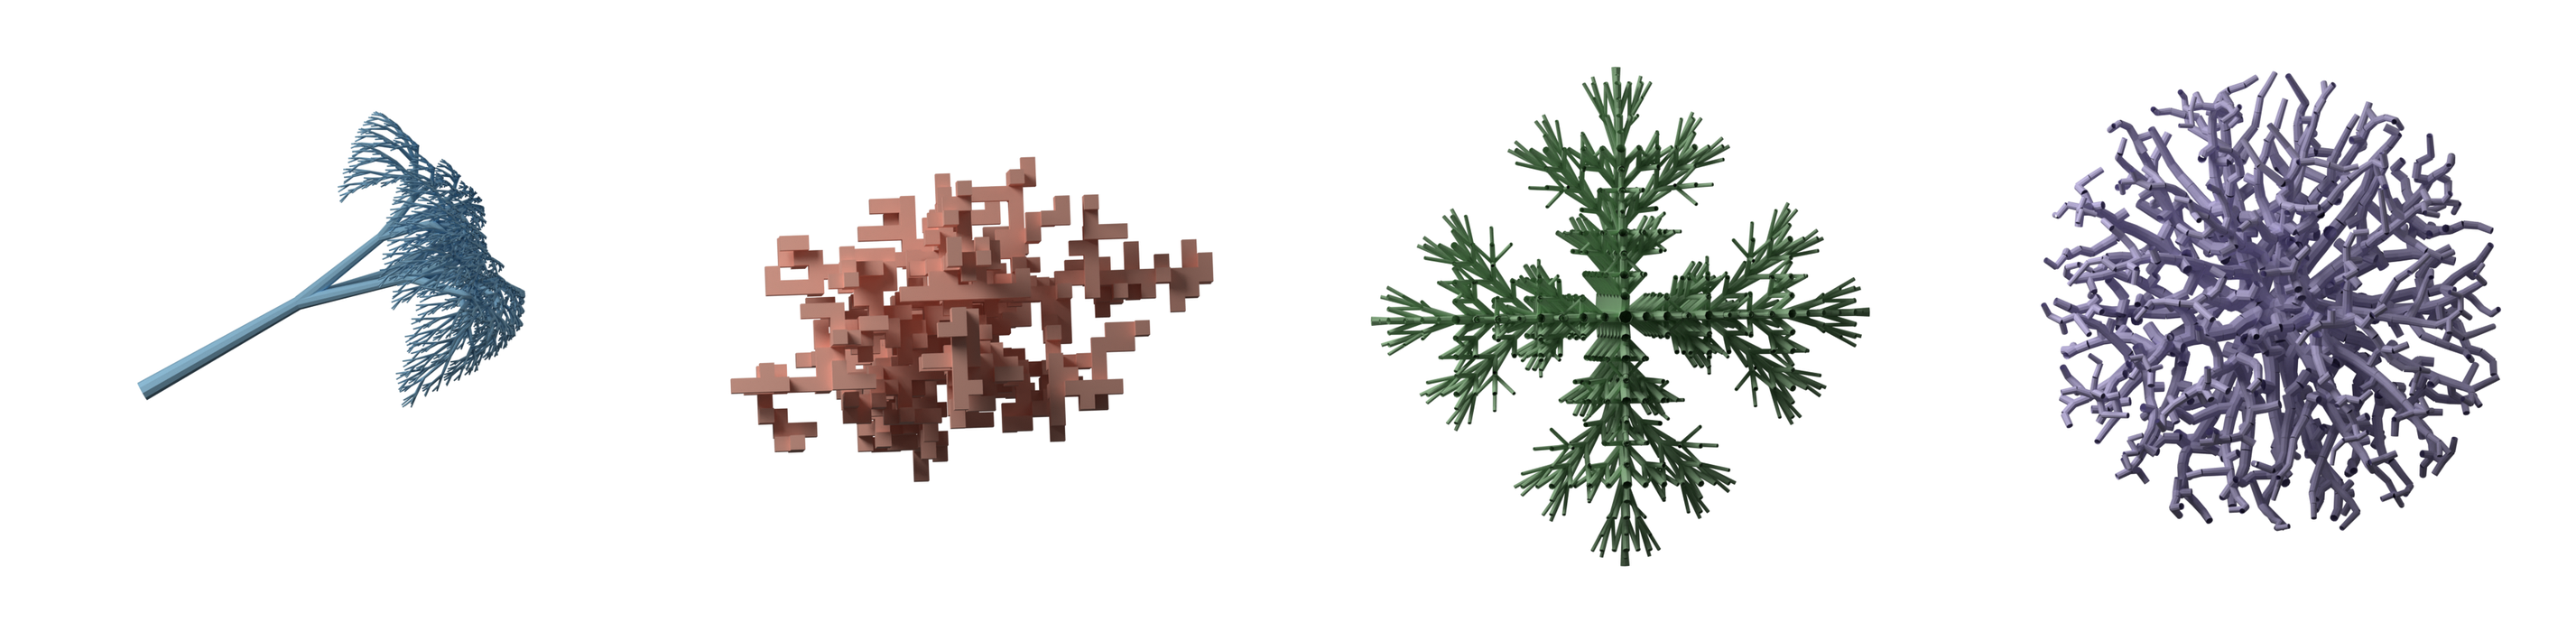
\includegraphics[width=\columnwidth]{figures/traditional_recursive_baselines_fourpanel_white_20260511.png}
  \Description{Four white-background renders of traditional procedural recursive baselines: an iterated-function-system branch structure, a diffusion-limited aggregation voxel cluster, an L-system branch structure, and a space-colonization tree canopy.}
  \caption{Traditional recursive controls rendered under a shared protocol: IFS transform-copy, DLA frontier accretion, L-system rewriting, and space-colonization growth.}
  \label{fig:traditional-recursive-baselines}
\end{figure}

\subsection{Learned Structure and Programmatic Shape Generation}

Learned structure and program models show the value of explicit 3D hierarchy. GRASS uses recursive autoencoders for hierarchical shape structures~\cite{grass2017}; StructureNet represents shapes as part graphs~\cite{structurenet2019}; and ShapeAssembly learns a domain-specific assembly language~\cite{shapeassembly2020} from object-family data such as PartNet~\cite{partnet2019}. We use user-authored finite-depth rules and execute their local edits through a frozen sparse latent generator while the resulting state remains addressable, attached, and reusable.

\subsection{Native 3D Generation and Sparse Latent 3D Generators}

Large-scale 3D datasets support strong learned priors for geometry realization~\cite{objaverse2023,objaverseXL2023}. Object-latent, set-latent, optimization-based, and feed-forward systems synthesize assets from compact codes, images, or text prompts~\cite{shapE2023,shape2vecset2023,poole2023dreamfusion,lin2023magic3d,chen2023fantasia3d,dreamgaussian2024,assetgen2024,hunyuan3d2025}. Sparse Latent 3D Generators expose token support, latent features, encoders, decoders, and local sampling paths~\cite{trellis2025,trellis2project}; our executor adds active handles, projection, and codec re-entry across depth.

\subsection{Sparse Editing and Structure-Conditioned Control}

Editing and control methods show that frozen generative priors can be reused locally. Flow editing and attention or feature-control methods redirect internal generative trajectories for localized changes~\cite{flowedit2025,hertz2022prompttoprompt,tumanyan2023plugandplay}; 3D editing methods modify NeRFs, voxel fields, or structured 3D latents while preserving selected regions~\cite{sella2023voxe,haque2023instructnerf2nerf,voxhammer2025,latte3d2025,nano3d2025,inpaintslat2026}; and structure-conditioned generation uses skeletons, point clouds, or geometric priors to guide native 3D synthesis~\cite{skadapter2026,pointsTo3D2026}. We use this local control inside a recursive executor: masked sparse-latent sampling realizes admitted local surface and feature edits, and projection converts each decoded candidate into an admissible state before later rules can read it.

\begin{figure}[t]
  \centering
  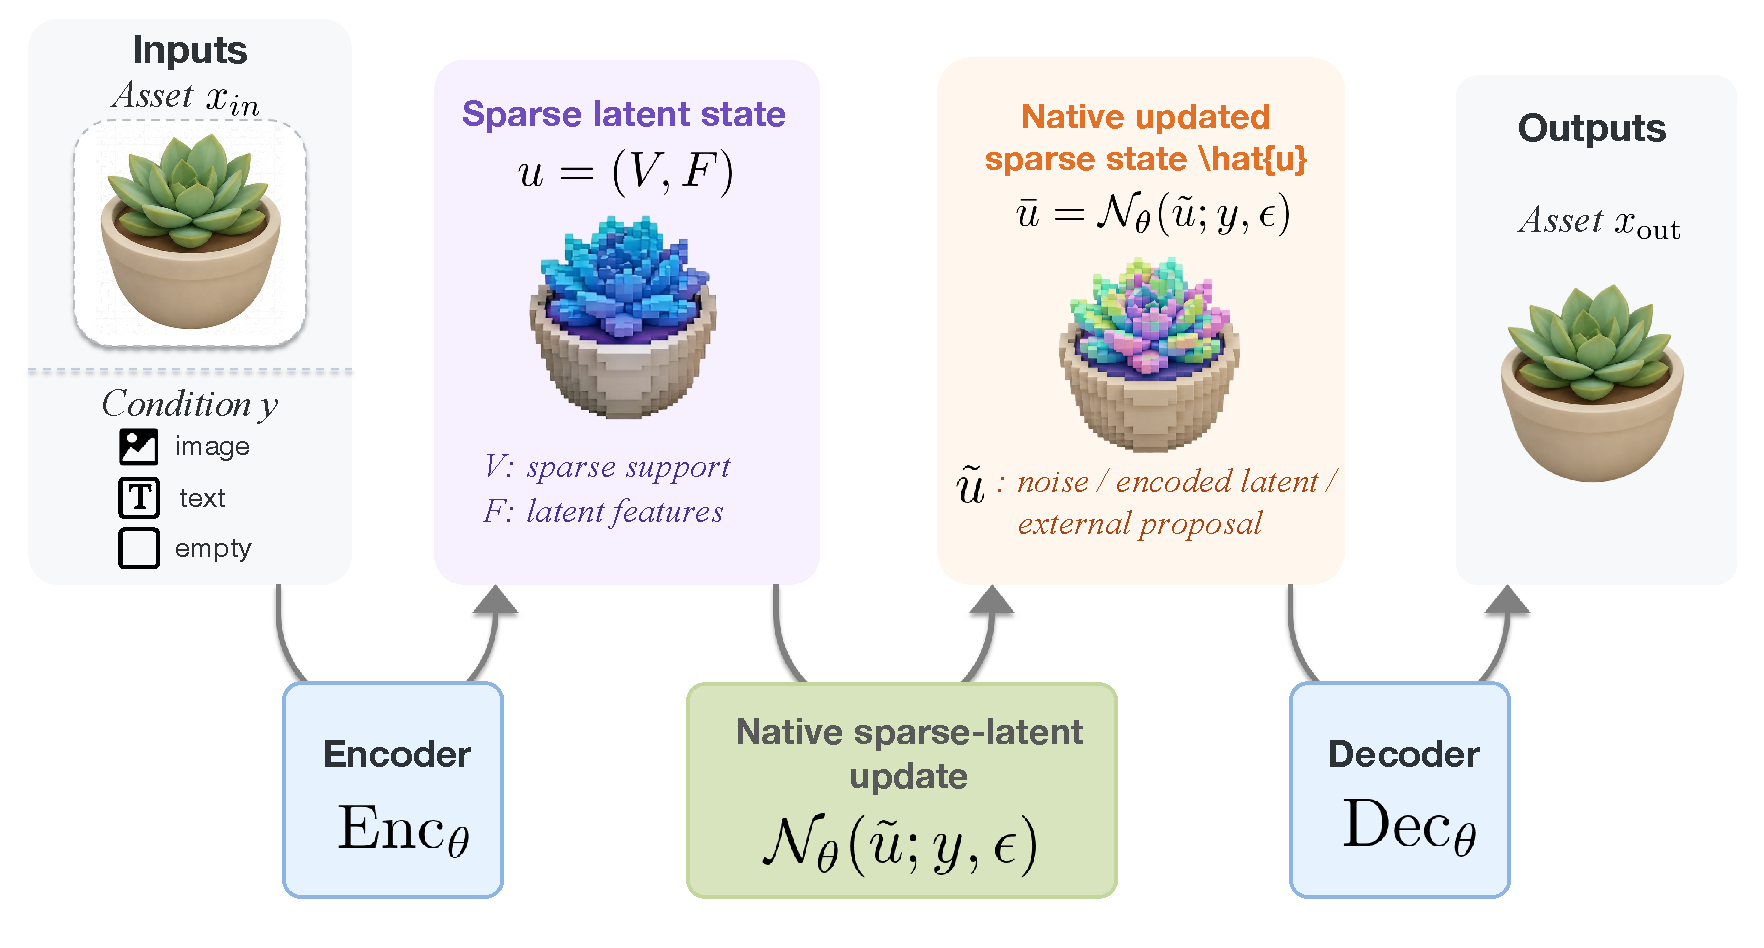
\includegraphics[width=\columnwidth]{figures/personal/sparse_latent_generator_interface_no_assets_editable.pdf}
  \Description{Compact sparse latent generator interface diagram showing a condition lane, optional input asset, encoder, sparse latent state, native sparse-latent sampler, decoder, and output 3D asset.}
  \caption{Frozen sparse latent generator interface: codec operations, sparse token support/features, native sparse-latent sampling, and decoding provide the substrate re-entered after projection.}
  \label{fig:sparse-latent-interface}
\end{figure}

\section{Preliminaries}
\begin{figure*}[t!]
  \centering
  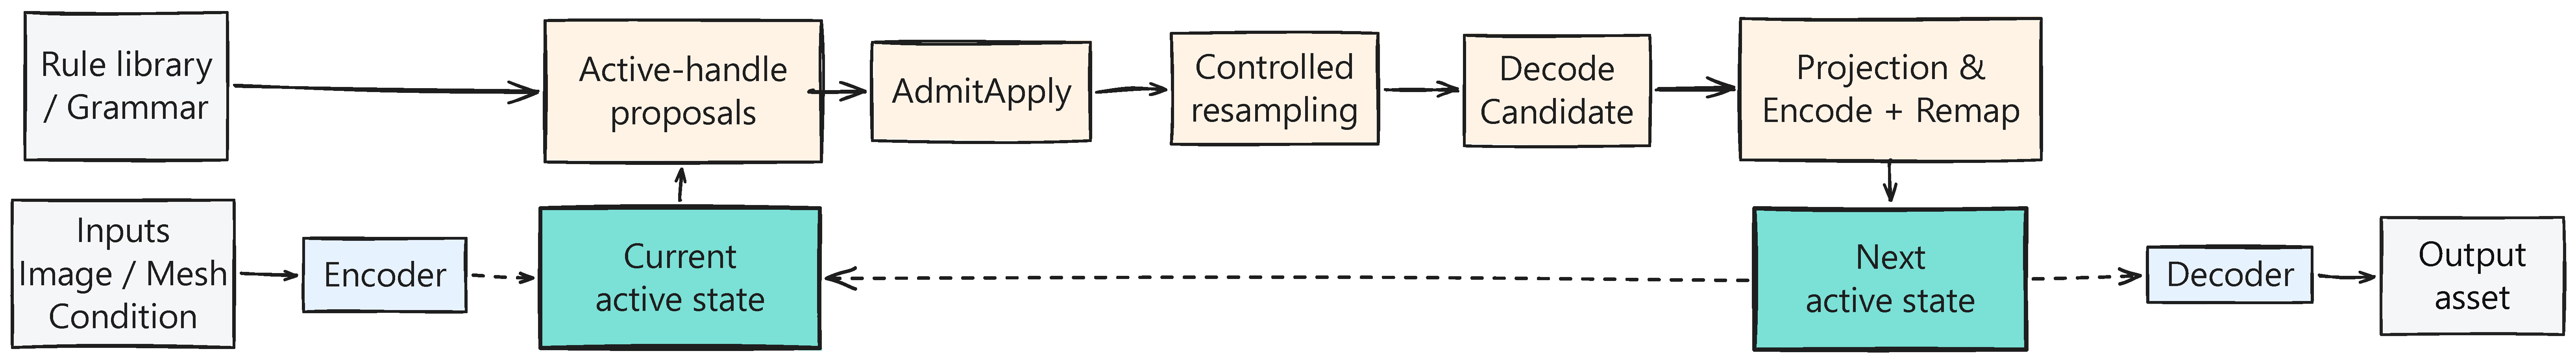
\includegraphics[width=\textwidth]{figures/personal/main_new.pdf}
  \Description{Layered overview diagram with a pretrained sparse latent generator interface on top and a recursive transition loop below, organized as proposal and admission, sparse-latent sampling and decoding, projection, and codec-closed commit.}
  \caption{The executor repeats rule proposal, admission, controlled sparse-latent resampling, decoding, projection, codec re-entry, and handle remapping before the next recursive depth reads the active state.}
  \label{fig:method-overview}
\end{figure*}
\subsection{Finite-Depth Recursive Programs}

We model recursive 3D asset generation as a finite-depth execution process whose committed state is read by later rules. A depth-$D$ execution is
\begin{equation}
s_{d+1}=\operatorname{Step}(s_d,\mathcal R_d,\xi_d),
\qquad
x_D=\operatorname{Output}(s_D),
\quad d=0,\ldots,D-1,
\end{equation}
where $\mathcal R_d\subseteq\mathcal R$ is the selected rule set and $\xi_d$ contains deterministic or stochastic choices. Executability means that $s_d$ stores handles, frontiers, motifs, or descriptors that later rules may read. Sec.~\ref{sec:program-state} instantiates this state as sparse generator tokens plus a root descriptor and handle registry.



\subsection{Sparse Latent Generator Interface}

Let $\theta$ denote a pretrained sparse latent 3D generator with fixed parameters. Its native sparse state is
\begin{equation}
u=(V,F),
\end{equation}
where $V\subset \delta_g\mathbb Z^3$ is sparse token support on generator grid spacing $\delta_g$ and $F:V\rightarrow\mathbb R^q$ stores token features. A condition $y$ may be an image, text-derived guide, category hint, material guide, or empty condition.

We use the generator through its sparse codec and native sparse-latent update:
\begin{equation}
u=\operatorname{Enc}_{\theta}(x,y),\qquad
\widehat u=\mathcal N_{\theta}(\tilde u;y,\epsilon),\qquad
x=\operatorname{Dec}_{\theta}(\widehat u,y).
\end{equation}
Here $\tilde u$ is the sparse latent sampler input, $\epsilon$ collects sampler choices, and $\mathcal N_{\theta}$ denotes the native diffusion or flow-matching update that returns model-consistent sparse state $\widehat u$.

The generator supplies sparse support, latent features, codec operations, and a learned realization prior. The executor adds active handles, proposal admission, controlled resampling, projection, and codec re-entry through the decode--project--re-encode--remap loop. In Sec.~\ref{sec:controlled-resampling}, $\operatorname{Resample}_\theta$ is the masked and anchored use of $\mathcal N_\theta$, and $\operatorname{FM}_\theta$ is the Trellis2 flow-matching instantiation.



\section{Method}

\subsection{Program State}
\label{sec:program-state}

The executor turns generator-native support and features into executable recursive state by adding a root descriptor and rule-readable handles. At depth $d$, the generator-native state is
\begin{equation}
u_d=(V_d,F_d),
\end{equation}
where $V_d\subset \delta_g\mathbb Z^3$ is sparse token support and $F_d:V_d\rightarrow\mathbb R^q$ stores token features. The recursive program state is
\begin{equation}
s_d=(u_d,r_d,A_d,m_d).
\end{equation}

The root descriptor is
\begin{equation}
r_d=(T_d^{\mathrm{root}},V_d^{\mathrm{root}},U_d^{\mathrm{root}},\beta_d).
\end{equation}
anchors the asset with a root frame, sparse root support, decoded root seeds, and family metadata. The metadata bundle $m_d$ stores connector certificates, token budgets, and projection thresholds carried between steps. The registry $A_d$ contains typed handles for trunks, crowns, frontiers, crystal cells, or reusable motif frames:
\begin{equation}
h_i=(\sigma_i,T_i,\Omega_i^{\mathrm{own}},\Omega_i^{\mathrm{tar}},\mu_i,b_i),
\end{equation}
where $\sigma_i$ is its type, $T_i$ a local frame, $\Omega_i^{\mathrm{own}}\subseteq V_d$ owned support, $\Omega_i^{\mathrm{tar}}\subseteq V_d$ target or reusable support, $\mu_i$ ownership/frontier/connector/reuse metadata, and $b_i\in\{0,1\}$ its active flag. Rules read
\begin{equation}
A_d^{\mathrm{act}}=\{h_i\in A_d:b_i=1\}.
\end{equation}

A handle is executable only when it is active, addressable in sparse support, and root-reachable or connector-certified. Let $V_d^{\mathrm{root}}\subseteq V_d$ be root support and let $G_\eta(V_d)$ be the $\eta$-neighborhood graph:
\begin{equation}
V_d^{\mathrm{att}}=
\{v\in V_d:\ \operatorname{path}_{G_\eta(V_d)}(v,V_d^{\mathrm{root}})\}.
\end{equation}
With threshold bundle $\lambda_d$ for attachment, frontier, connector, budget, and projection tolerances, committed connector support $C_d^{\mathrm{com}}\subseteq V_d$ is stored in $m_d$ after the previous projection. Admissibility requires active owned support in $V_d^{\mathrm{att}}\cup C_d^{\mathrm{com}}$, unique active ownership, token-budget compliance, and valid frontiers:
\begin{equation}
\begin{aligned}
\mathcal S_{\mathrm{adm}}(\lambda_d)
=
\{(u_d,r_d,A_d,m_d):\ C_1\land C_2\land C_3\land C_4\},
\end{aligned}
\end{equation}
with constraints
\begin{equation}
\begin{aligned}
C_1 &: \Omega_i^{\mathrm{own}}\subseteq
V_d^{\mathrm{att}}\cup C_d^{\mathrm{com}}
\quad \forall h_i\in A_d^{\mathrm{act}},\\
C_2 &: o_d(v)\ \text{is unique for every active owned } v,\\
C_3 &: |V_d|\le T_{\max}(d),\\
C_4 &: \operatorname{viol}_{\mathrm{frontier}}(s_d;\lambda_d)=0.
\end{aligned}
\end{equation}
Here $o_d$ is the active-support ownership map and $\operatorname{viol}_{\mathrm{frontier}}$ counts active frontier violations. The invariant is direct: later rules select only from $A_d^{\mathrm{act}}$.

\subsection{Rule Proposals and Admission}

Rules operate on the access layer defined by active handles. At depth $d$, the rule library reads handles in $A_d^{\mathrm{act}}$ and emits proposal records describing local sparse-state changes:
\begin{equation}
\mathcal P_d=\bigcup_{h_i\in A_d^{\mathrm{act}}}\rho(h_i;s_d),
\qquad
p_j=(\Delta V_j,\Delta F_j^{\mathrm{seed}},H_j,\mu_j).
\end{equation}
Here $\Delta V_j$ proposes support edits, $\Delta F_j^{\mathrm{seed}}$ provides feature seeds or copied features, $H_j$ stores handle records, and $\mu_j$ records attachment, mask, connector, priority, budget, ownership, and compatibility metadata. Deterministic admission orders proposals, resolves mergeable conflicts, writes accepted metadata into $\widetilde A_{d+1}$, and records feasibility certificates in $\Gamma_d$. The same interface supports branching, frontier-growth, transform-copy, and split/extrude families; Appendix~\ref{app:moved-main-tables} gives the vocabulary map, and Fig.~\ref{fig:one-branch} illustrates one branch transition.

\begin{figure}[t]
  \centering
  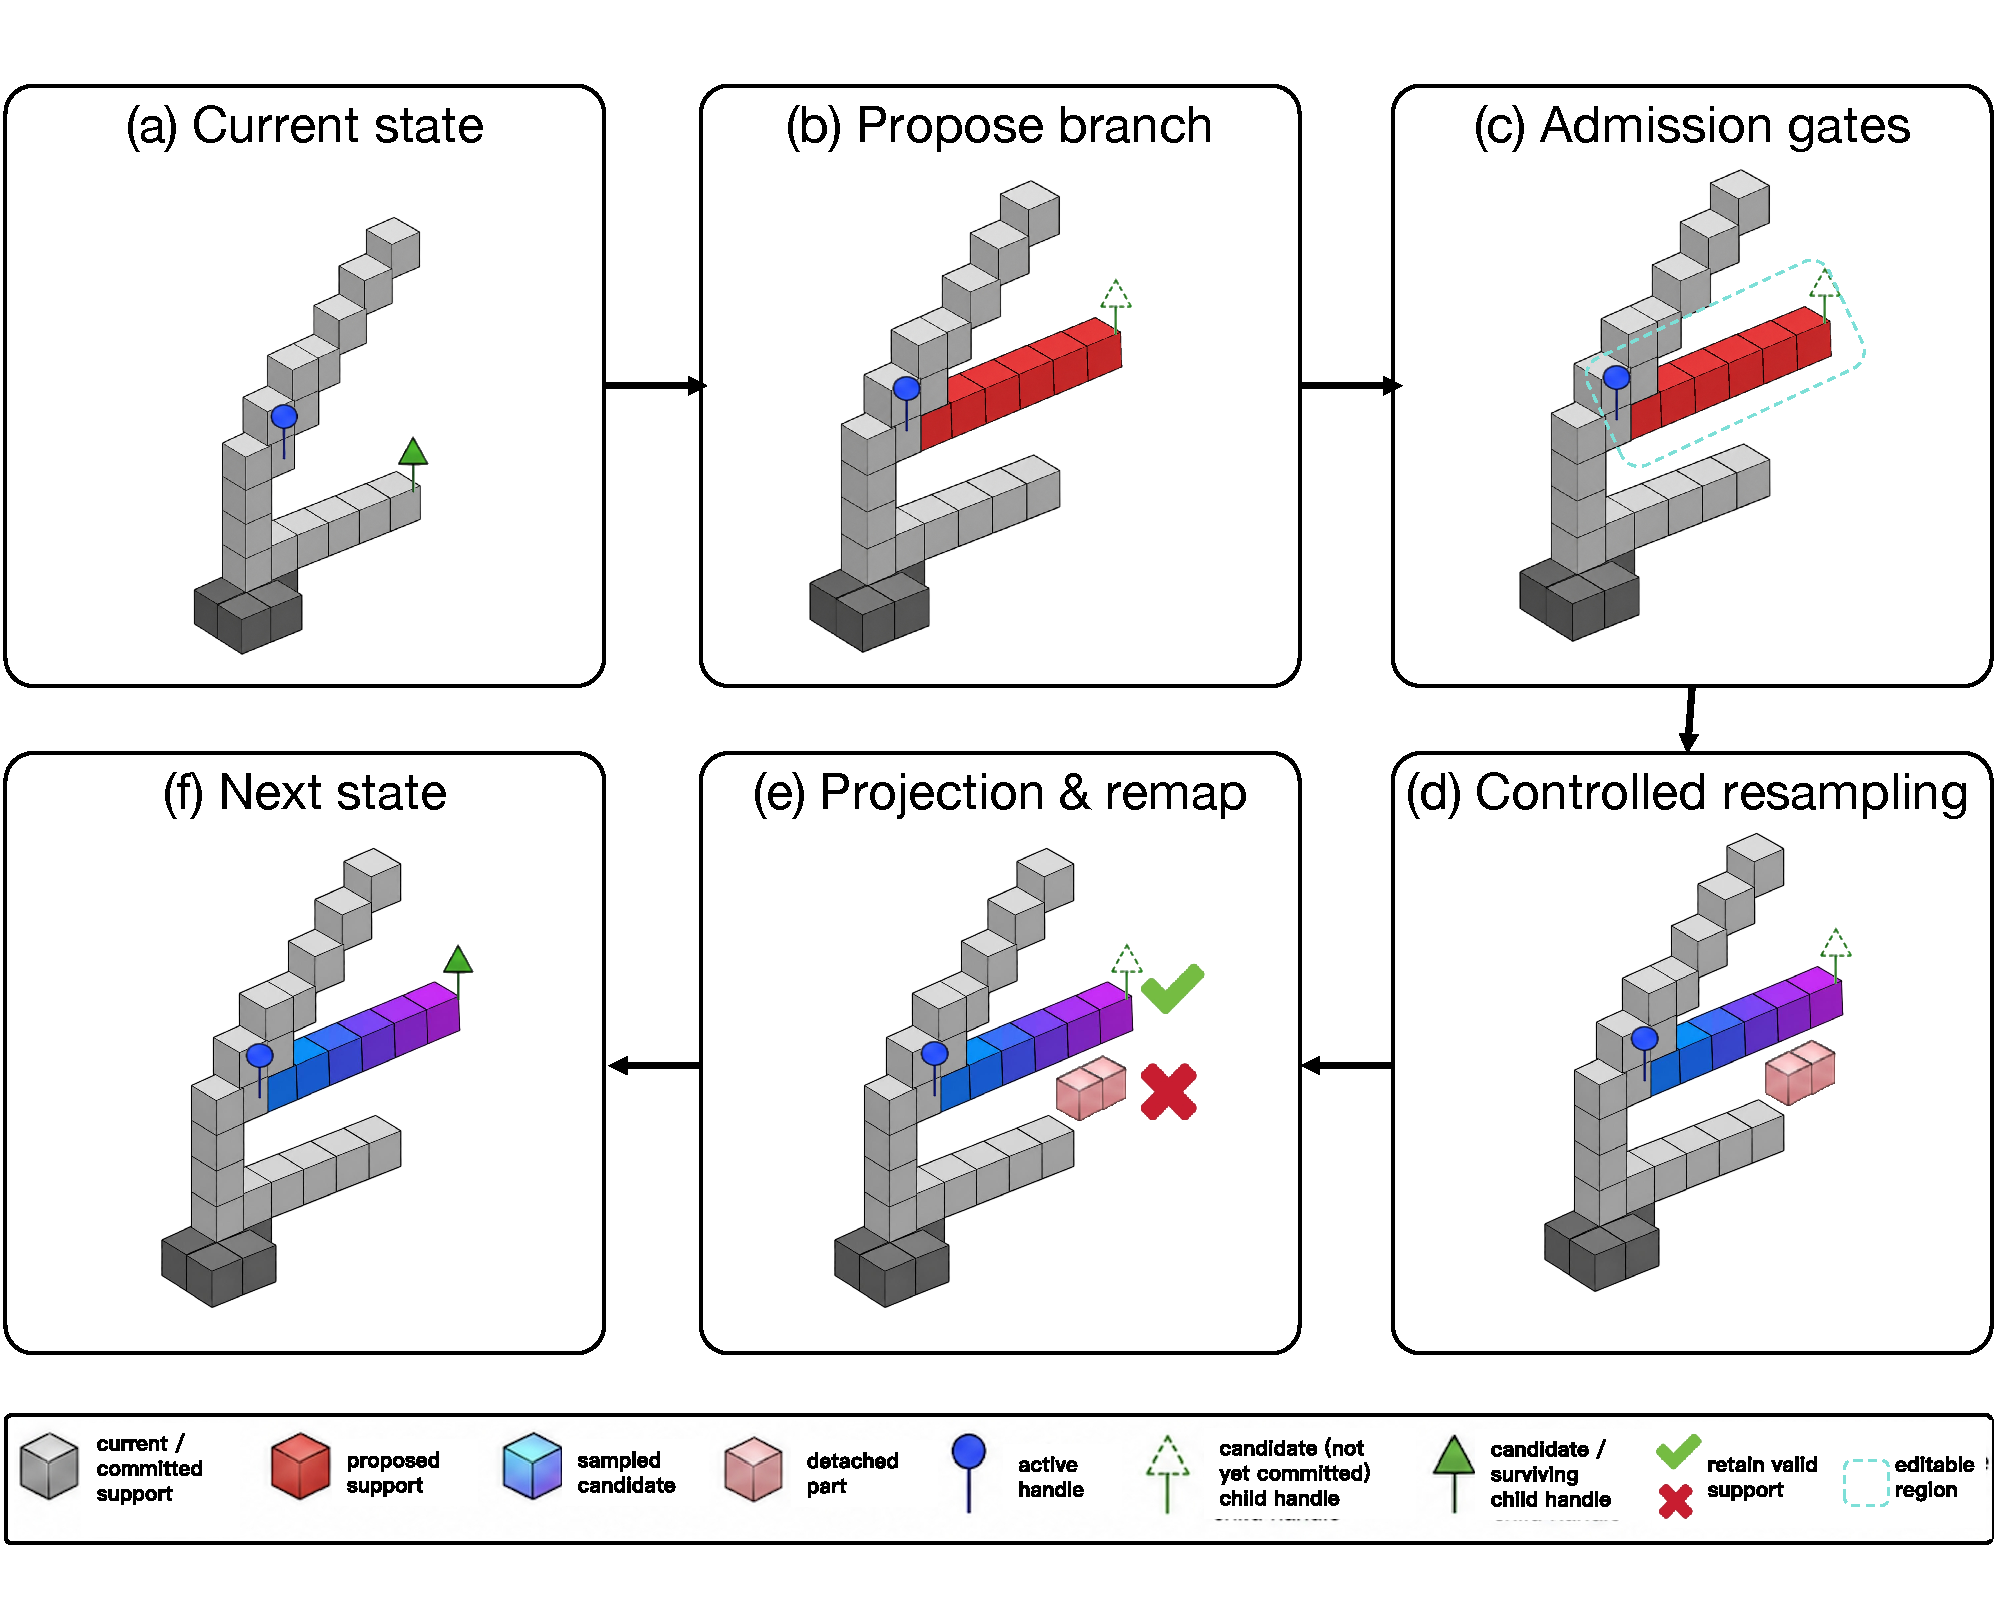
\includegraphics[width=\columnwidth]{figures/personal/stick_case_new.pdf}
  \Description{One recursive branch transition: an active parent handle proposes a child support region, the sparse latent generator realizes the local candidate, and projection removes detached support before the next state is committed.}
  \caption{One branch transition: admission gates accept a child proposal; controlled sparse-latent sampling realizes it; projection, codec re-entry, and handle remapping commit the next active state.}
  \label{fig:one-branch}
\end{figure}

\subsection{Projection-Stabilized Recursive Transition}

A transition maps the current executable state to the next one:
\begin{equation}
s_{d+1}
=
\mathcal T_\theta(s_d;\mathcal R,y,\lambda_d,\psi_d).
\end{equation}
Given root asset $x_0$, condition $y$, rules $\mathcal R$, and depth $D$, the executor initializes
\begin{equation}
u_0=\operatorname{Enc}_{\theta}(x_0,y),
\qquad
s_0=(u_0,r_0,A_0,m_0),
\end{equation}
where $r_0$ stores the root descriptor, $A_0$ stores root handles and growth frames, and $m_0$ stores initial connector and budget metadata.

At depth $d$, the transition is organized as four operational stages before codec-closed commit. First, rules read the active state and emit symbolic proposals:
\begin{equation}
\mathcal P_d=\operatorname{Propose}(s_d,\mathcal R).
\end{equation}
These records describe intended growth, reuse, or frontier updates.

Second, admission turns proposals into a sparse edit with masks, anchors, and feasibility certificates:
\begin{equation}
(\widetilde u_{d+1},\widetilde A_{d+1},M_d,B_d,\Gamma_d)
=
\operatorname{AdmitApply}(\mathcal P_d,s_d,\lambda_d).
\end{equation}
Here $M_d$ marks editable support, $B_d$ stores anchors, and $\Gamma_d$ records attachment evidence.

Third, masked-and-anchored resampling realizes the admitted edit and decoding exposes it for geometric evaluation:
\begin{equation}
\bar u_{d+1}
=
\operatorname{Resample}_\theta
(\widetilde u_{d+1};y,M_d,B_d,\psi_d),
\qquad
x_{d+1}
=
\operatorname{Dec}_{\theta}(\bar u_{d+1},y).
\end{equation}
Projection then converts the realized geometry into reusable recursive state.

Fourth, projection keeps root-attached support, revises handles, and returns codec correspondence:
\begin{equation}
(x^\star_{d+1},r_{d+1},\widehat A_{d+1},\kappa_{d+1})
=
\Pi_{\lambda_d}(x_{d+1},\widetilde A_{d+1},s_d,\Gamma_d).
\end{equation}
The commit re-enters the sparse latent codec and exposes remapped handles to the next depth:
\begin{equation}
\begin{aligned}
u_{d+1}
&=
\operatorname{Enc}_{\theta}(x^\star_{d+1},y),\\
A_{d+1}
&=
\operatorname{Remap}
(\widehat A_{d+1},\kappa_{d+1},V_{d+1}),\\
s_{d+1}
&=
(u_{d+1},r_{d+1},A_{d+1},m_{d+1}).
\end{aligned}
\end{equation}
The policy $\psi_d$ selects the sampling schedule and correspondence rule, while $m_{d+1}$ stores the committed connector certificates and projection metadata for the next transition.

Thus projection is an admissibility gate inside the recursive transition: it selects decoded support and surviving handles, while codec re-entry materializes $V_{d+1}$ and remaps handle support before later rules read $A_{d+1}^{\mathrm{act}}$. Every active parent, frontier, connector, or reusable motif at depth $d+1$ has passed projection before reuse.

\begin{algorithm}[t]
  \caption{Formal codec-closed PS-RSLE transition with per-depth projection.}
  \label{alg:ps-rsle-execution}
  \begin{algorithmic}[1]
    \Require root asset $x_0$, rules $\mathcal R$, condition $y$, depth $D$, projection schedule $\{\lambda_d\}$, resampling policies $\{\psi_d\}$
    \Ensure projected state $s_D$ and final projected asset $x_D^\star$

    \State $u_0 \gets \operatorname{Enc}_\theta(x_0,y)$
    \State initialize handle registry $A_0$
    \State initialize root descriptor $r_0$
    \State initialize metadata bundle $m_0$
    \State $s_0\gets(u_0,r_0,A_0,m_0)$

    \For{$d=0,\ldots,D-1$}
      \State $\mathcal P_d \gets \operatorname{Propose}(s_d,\mathcal R)$
      \State $(\widetilde u_{d+1},\widetilde A_{d+1},M_d,B_d,\Gamma_d)
      \gets \operatorname{AdmitApply}(\mathcal P_d,s_d,\lambda_d)$
      \State $\bar u_{d+1}
      \gets \operatorname{Resample}_\theta(\widetilde u_{d+1};y,M_d,B_d,\psi_d)$
      \State $x_{d+1}\gets \operatorname{Dec}_\theta(\bar u_{d+1},y)$
      \State $(x^\star_{d+1},r_{d+1},\widehat A_{d+1},\kappa_{d+1})
      \gets \Pi_{\lambda_d}(x_{d+1},\widetilde A_{d+1},s_d,\Gamma_d)$
      \State $u_{d+1}\gets \operatorname{Enc}_\theta(x^\star_{d+1},y)$
      \State $A_{d+1}\gets \operatorname{Remap}(\widehat A_{d+1},\kappa_{d+1},V_{d+1})$
      \State update metadata bundle $m_{d+1}$
      \State $s_{d+1}\gets(u_{d+1},r_{d+1},A_{d+1},m_{d+1})$
    \EndFor

    \State $x_D^\star\gets x^\star_D$
    \State \Return $s_D$, $x_D^\star$
  \end{algorithmic}
\end{algorithm}

Algorithm~\ref{alg:ps-rsle-execution} specifies the codec-closed semantics used throughout the experiments and isolated by the projection ablation in Sec.~\ref{sec:projection-ablation}.

\subsection{Controlled Sparse-Latent Resampling}
\label{sec:controlled-resampling}

Rule proposals edit sparse support and seed features. The executor uses the generator's native sparse-latent flow sampler to realize admitted local proposals before decoding and projection. In the implementation evaluated here, controlled resampling freezes admitted support $\widetilde V_{d+1}$ and updates token features; decoded support changes are handled by projection and codec re-entry. The local flow and masked blend are
\begin{equation}
\begin{aligned}
\frac{d u_t}{dt}
&=v_\theta(u_t,t,y),\\
u^\theta_{d+1}
&=(V^\theta_{d+1},F^\theta_{d+1})
=\operatorname{FM}_\theta(\widetilde u_{d+1};y,\psi_d),\\
\bar F_{d+1}(v)
&=
\begin{cases}
\widetilde F_{d+1}(v), & v\notin M_d,\\
(1-\alpha_v)\widetilde F_{d+1}(v)+\alpha_v F^\theta_{d+1}(\chi(v)),
& v\in M_d .
\end{cases}
\end{aligned}
\end{equation}
Here $\chi(v)$ is the sparse correspondence from admitted editable support to sampled support, using identity matches when present and nearest valid sparse-grid correspondence otherwise. Sparse transforms are discretized on the generator grid before this merge: transformed coordinates are rounded to sparse-grid locations, invalid coordinates are clipped, and duplicate coordinates are merged by averaging their features.
Anchors are hard-clamped by setting $\alpha_v=0$ for $v\in B_d$, so boundary and root support specified by admission remain fixed inside the masked-and-anchored resampling call.

For copied motifs, rules may also supply a source--target correspondence $\pi$ for feature reuse:
\begin{equation}
\bar F_{d+1}(v)
\leftarrow
(1-\gamma_v)F^{\theta}_{d+1}(v)
+\gamma_v F^{\mathrm{src}}(\pi(v)).
\end{equation}
The resampled sparse latent $\bar u_{d+1}=(\widetilde V_{d+1},\bar F_{d+1})$ is then decoded:
\begin{equation}
x_{d+1}
=
\operatorname{Dec}_{\theta}(\bar u_{d+1},y).
\end{equation}
This step realizes local geometry and feature continuity under the frozen generator prior; projection then commits the executable parents, frontiers, connectors, and reusable motifs.

\subsection{Projection}

Admissibility projection is the commit step of the executor. Given decoded realization $x_{d+1}$, proposed handles $\widetilde A_{d+1}$, previous state $s_d$, admission certificates $\Gamma_d$, and thresholds $\lambda_d$, projection computes
\begin{equation}
(x^\star_{d+1},r_{d+1},\widehat A_{d+1},\kappa_{d+1})
=
\Pi_{\lambda_d}(x_{d+1},\widetilde A_{d+1},s_d,\Gamma_d).
\end{equation}

Projection is performed in the decoded domain, where component membership and root reachability are evaluated on the realized shape. The executor samples or voxelizes $x_{d+1}$ to obtain support $U$, builds $G_\eta(U)$, and instantiates root seeds $U^{\mathrm{root}}\subseteq U$ from the persistent root descriptor:
\begin{equation}
U^{\mathrm{att}}
=
\{u\in U:\operatorname{path}_{G_\eta(U)}(u,U^{\mathrm{root}})\}.
\end{equation}
Support in $U^{\mathrm{att}}$, together with connector support whose certificates in $\Gamma_d$ satisfy endpoint attachment, mask validity, collision clearance, and budget tolerances, becomes eligible active support. Child, frontier, connector, and motif handles survive when their realized support satisfies attachment, ownership, frontier, and token-budget constraints.

Projection first produces decoded support $U^\star\subseteq U$, a projected decoded handle registry $\widehat A_{d+1}$, and decoded correspondence records used by codec re-entry. Re-encoding yields sparse support $V_{d+1}$ and finalizes the correspondence $\kappa_{d+1}:U^\star\rightarrow V_{d+1}$; $\operatorname{Remap}$ then updates surviving handles through declared proposal transforms, overlap with projected support, or $\kappa_{d+1}$. This handle update is what makes projection a state operation rather than a geometry-only cleanup step.

In the codec-closed semantics, the projected asset is re-encoded by the generator codec in the outer transition, producing $u_{d+1}=\operatorname{Enc}_\theta(x^\star_{d+1},y)$ and the committed state $s_{d+1}=(u_{d+1},r_{d+1},A_{d+1},m_{d+1})$ after handle remapping and metadata update. This decode--project--re-encode--remap loop evaluates connectivity and ownership in the realized domain, then returns to generator-native sparse state before later rules read the active subset. Appendix~\ref{app:projection-routine} gives the operational projection routine used by the executor.

\section{Experiments}

\subsection{Experimental Setup}
\paragraph{Tasks.}
We evaluate finite-depth recursive 3D asset tasks spanning branching assets, frontier-growth assets, and transform-copy assets. These tasks test root-attached expansion, repeated attachment under dense local support, reusable motifs, and depth-controlled structure with a training-free executor around a frozen sparse latent 3D generator.

\paragraph{Baselines.}
Baselines include traditional L-system, space-colonization, DLA/frontier, and IFS/transform programs with strong explicit recursive structure~\cite{lindenmayer1968lsystemsI,prusinkiewicz1990abop,runions2007spacecolonization,witten1981dla,sander2000dlaReview,hutchinson1981fractals,barnsley1988fractalsEverywhere}, plus Trellis2 one-shot, Trellis2 latent-copy, Trellis2 generated-root mesh-copy, and Hunyuan3D generated-root mesh-copy controls~\cite{trellis2025,trellis2project,hunyuan3d2025}. Together they separate terminal object synthesis from recursive execution over editable intermediate state.

\paragraph{Metrics.}
Metrics cover the paper's three claims: connected support through occupancy and surface LCR, executable state through root reachability, orphan handles, handle survival, and valid execution rate, and local realization through welded components, open edges, roughness, normal consistency, artifact score, and deterministic proxy score. Appendix~\ref{app:moved-main-tables} records task-to-rule coverage and matched protocols.

\subsection{Comparison with Traditional Procedural Methods}
\label{sec:traditional-comparison}
Figure~\ref{fig:main-experiment-traditional-vs-ours} and Table~\ref{tab:main-experiment-selected-metrics} compare our method with traditional procedural controls under matched target families. The procedural controls retain strong explicit structure, while our method adds generator-realized surface detail and natural asset appearance. Our DLA/frontier and IFS/transform rows are single-component under the strict surface metric, and the space-colonization and L-system rows keep high largest-component ratios of $0.996$ and $0.979$. The method also reduces welded fragmentation in the space-colonization, L-system, and IFS/transform rows, with welded component counts of $1$, $9$, and $1$ compared with $627$, $508$, and $15$ for the corresponding procedural controls. In the DLA/frontier row, both methods reach one welded component, and our method adds a coral-like realized surface with richer local detail.
\begin{figure}[t]
  \centering
  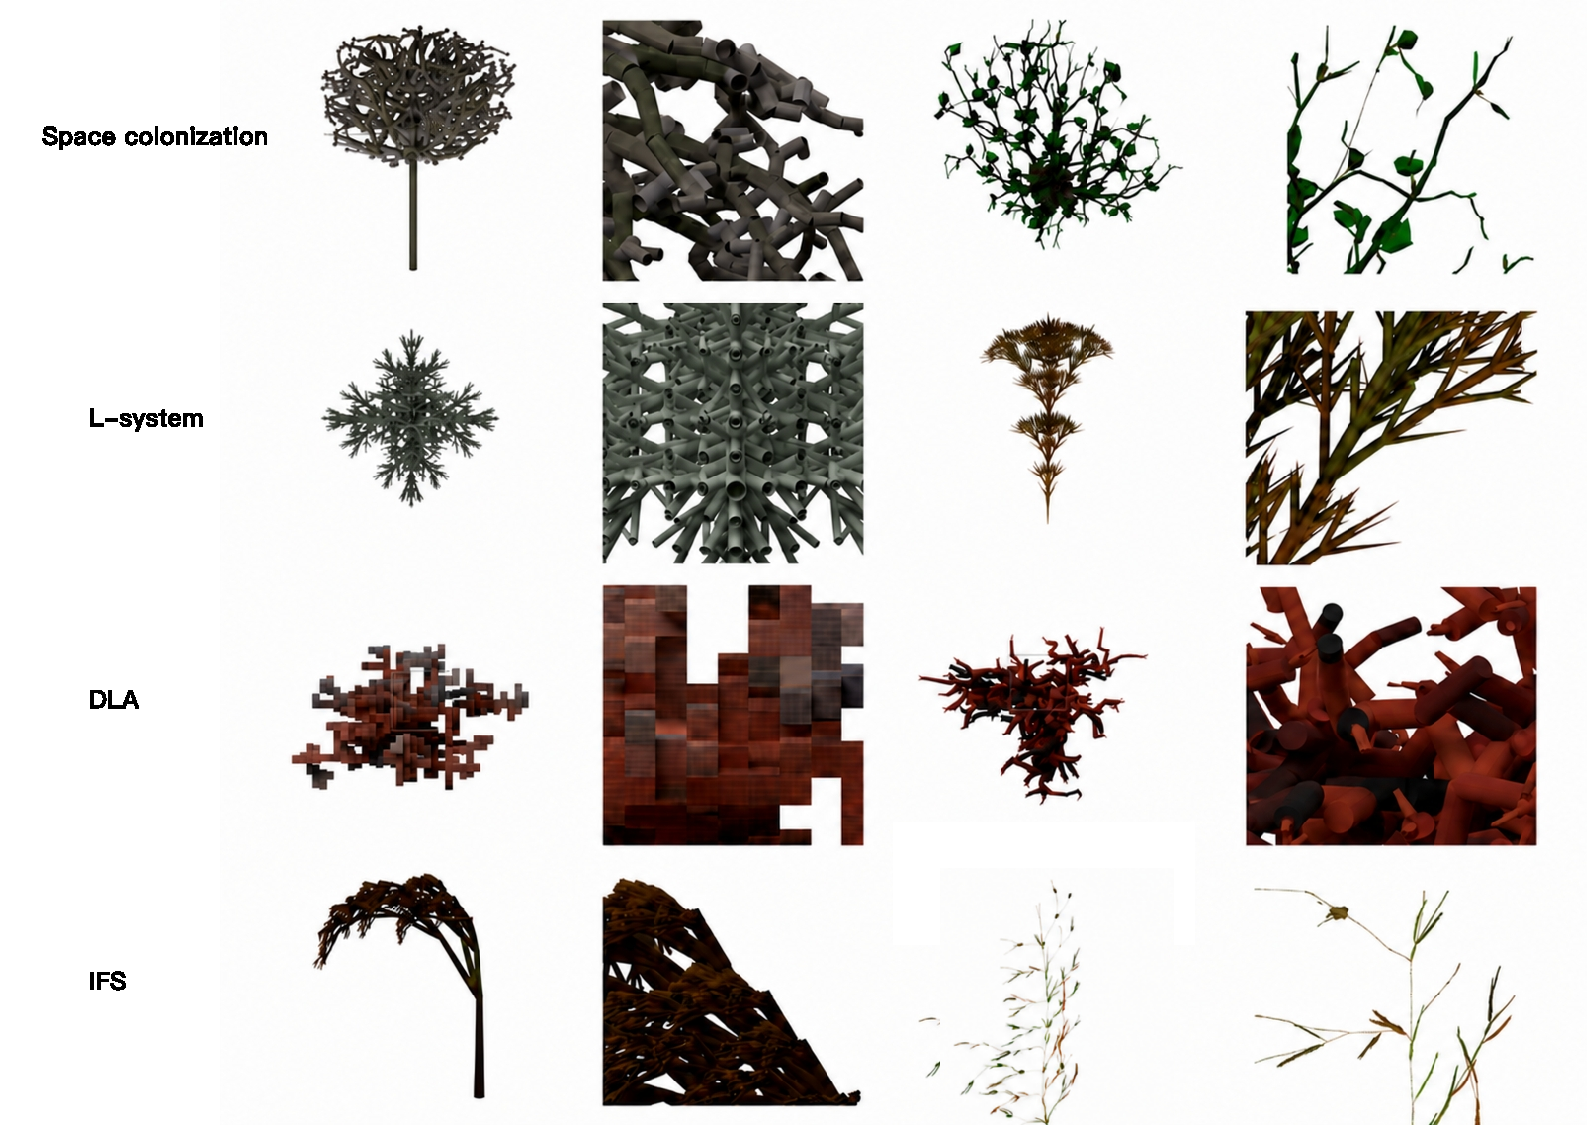
\includegraphics[width=\columnwidth]{figures/personal/Traditional_Compare_PPT.pdf}
  \Description{Four-row, four-column white-background comparison matrix. Rows show space-colonization, L-system, DLA/frontier, and IFS/transform branch targets. Columns show traditional overview, traditional zoom-in, our overview, and our zoom-in.}
  \caption{Traditional procedural controls and our assets compared under the same white-background overview and zoom protocol.}
  \label{fig:main-experiment-traditional-vs-ours}
\end{figure}

% Auto-generated by assets/write_main_experiment_metrics_table_corrected_V67B_20260512.py
\begin{table}[t]
\centering
\scriptsize
\setlength{\tabcolsep}{2pt}
\caption{Traditional comparison with strict surface connectivity, surface largest-component ratio, and welded fragmentation for space-colonization, L-system, DLA/frontier, and IFS/transform families~\cite{runions2007spacecolonization,lindenmayer1968lsystemsI,prusinkiewicz1990abop,witten1981dla,sander2000dlaReview,hutchinson1981fractals,barnsley1988fractalsEverywhere}.}
\label{tab:main-experiment-selected-metrics}
\resizebox{\columnwidth}{!}{%
\begin{tabular}{llrrr}
\toprule
Family & Method & Surf. comps. ($r=0$) & Surf. LCR ($r=0$) & Welded comp. \\
\midrule
Space colonization & Traditional & 1 & 1.000  & 627 \\
Space colonization & Ours & 6 & 0.996  & 1 \\
\addlinespace
L-system & Traditional & 6 & 0.999  & 508 \\
L-system & Ours & 107 & 0.979  & 9 \\
\addlinespace
DLA/frontier & Traditional & 6 & 1.000  & 1 \\
DLA/frontier & Ours & 1 & 1.000  & 1 \\
\addlinespace
IFS/transform & Traditional & 1 & 1.000  & 15 \\
IFS/transform & Ours & 1 & 1.000  & 1 \\
\bottomrule
\end{tabular}
}
\end{table}


\subsection{Comparison with 3D Generation and Mesh-Space Recursion}
\label{sec:experiment3-sparse-latent-vs-mesh-space}
Table~\ref{tab:experiment3-sparse-latent-vs-mesh-space} compares our method with one-shot generation and generated-root mesh-copy recursion. One-shot generation focuses on terminal object synthesis, while our method exposes editable recursive state for the next rule. Mesh-space recursion reuses generated roots through repeated copy-and-transform operations; Trellis2 generated-root mesh-copy gives $32$, $53$, $43$, and $46$ occupancy components on the four main cases, and Hunyuan3D generated-root mesh-copy gives $40$, $22$, $3$, and $3$. Ours returns one occupancy component on tree crown, bismuth, and coral, and three on pyrite, with LCR equal to $1.000$ in all four cases. Recursive execution in sparse latent space preserves connected occupied support most consistently across the comparison.
\begin{figure}[t]
  \centering
  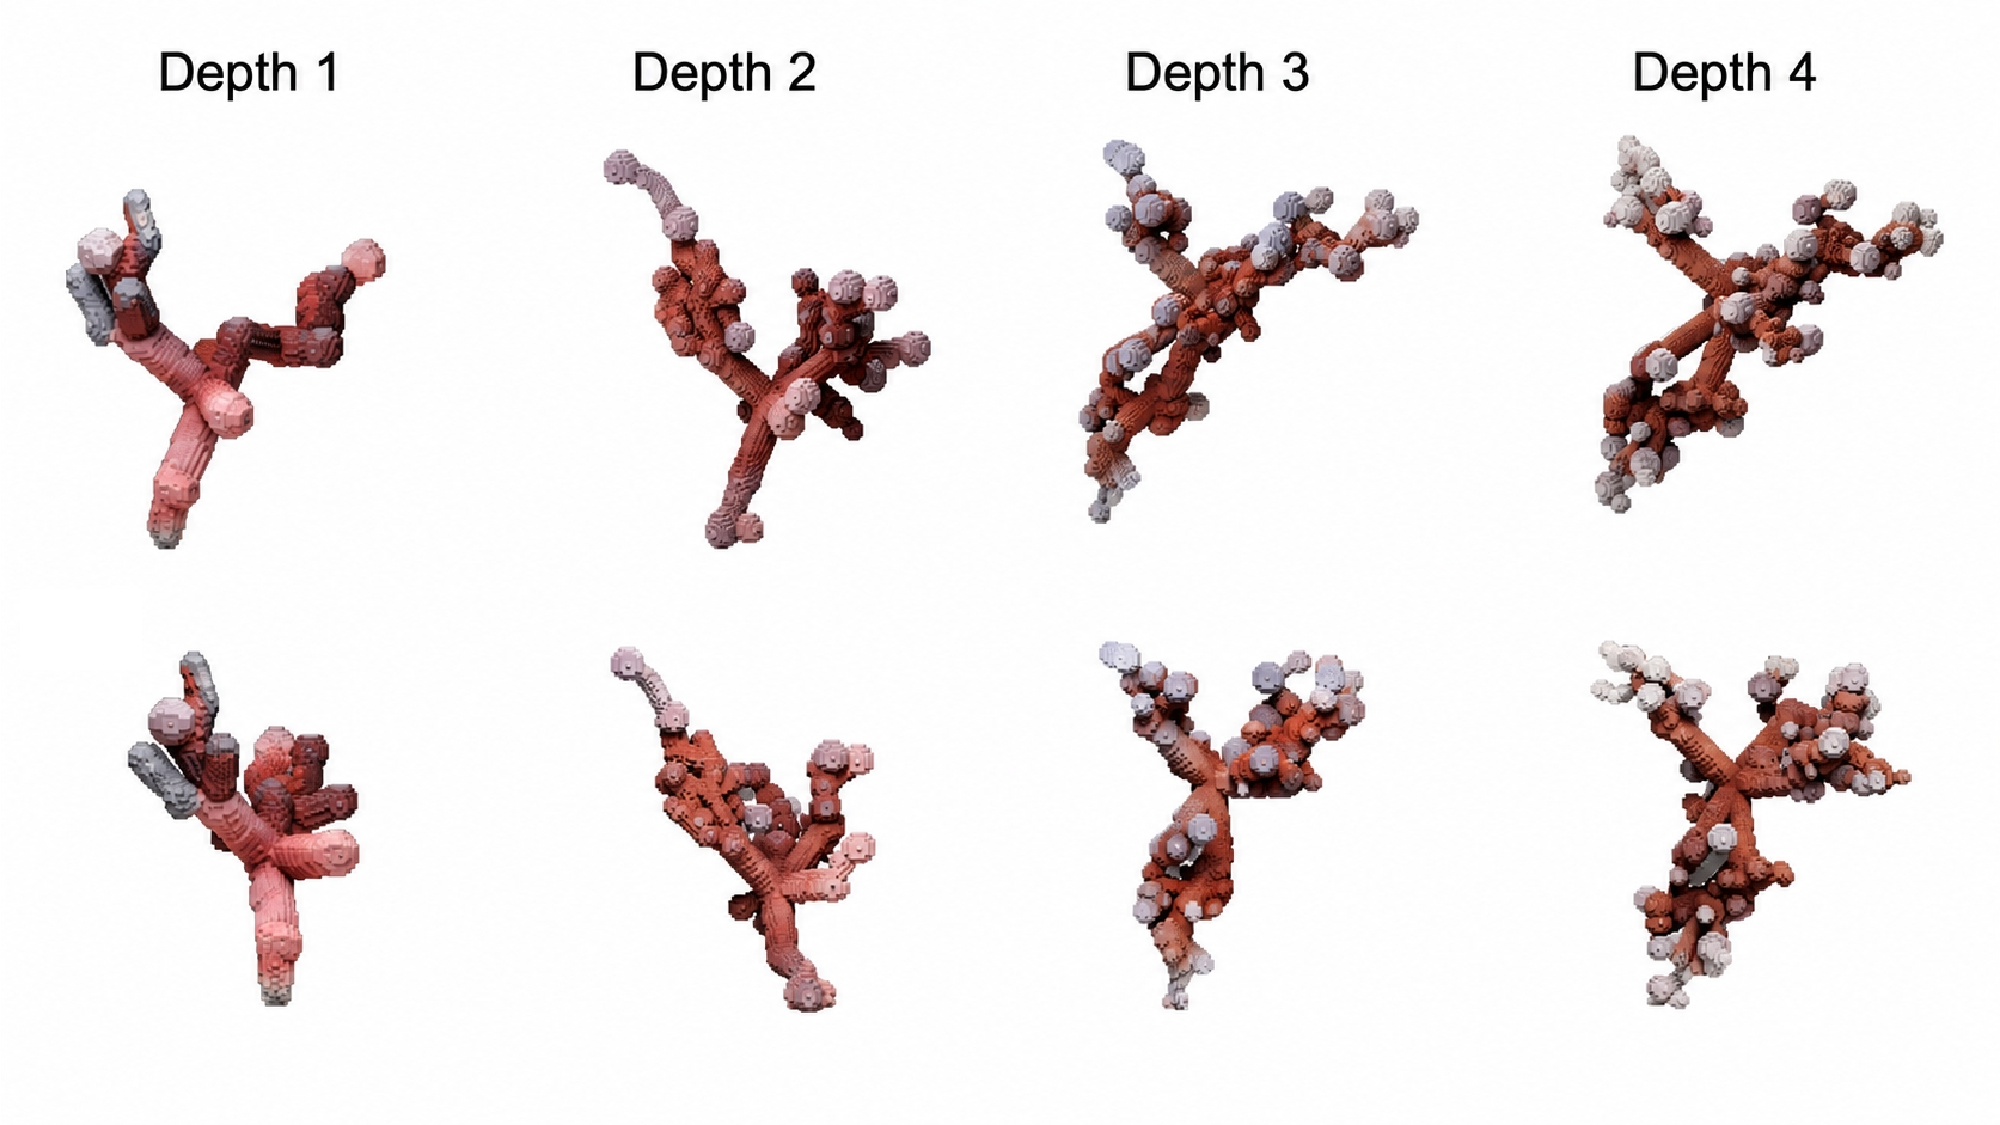
\includegraphics[width=\columnwidth]{figures/personal/coral_depth.pdf}
  \Description{Depth-control showcase for a coral or DLA-inspired connected scaffold with rendered branches.}
  \caption{Depth control on a connected coral-inspired frontier scaffold under a fixed rule family and rendering protocol.}
  \label{fig:coral-depth-textured}
\end{figure}
% Derived from results/experiment3_sparse_latent_vs_meshspace_20260511/experiment3_master_manifest.csv;
% compacted for the main paper.
\begin{table}[t]
\centering
\scriptsize
\setlength{\tabcolsep}{2.4pt}
\resizebox{0.90\columnwidth}{!}{\begin{tabular}{llrrrr}
\toprule
Case & Method & Occ. comp. & LCR & Welded comp. & Open edges \\
\midrule
tree crown & Trellis2 one-shot & 19 & 0.978 & -- & -- \\
tree crown & Trellis2 latent-copy & 11 & 0.995 & -- & -- \\
tree crown & Trellis2 mesh-copy & 32 & 0.993 & 48,931 & 466,284 \\
tree crown & Hunyuan3D mesh-copy & 40 & 0.998 & 90,895 & 467,428 \\
tree crown & Ours & 1 & 1.000 & 169 & 96,428 \\
\midrule
bismuth & Trellis2 one-shot & 1 & 1.000 & -- & -- \\
bismuth & Trellis2 latent-copy & 7 & 0.909 & -- & -- \\
bismuth & Trellis2 mesh-copy & 53 & 0.112 & 132,816 & 897,700 \\
bismuth & Hunyuan3D mesh-copy & 22 & 0.999 & 256,216 & 898,400 \\
bismuth & Ours & 1 & 1.000 & 179 & 15,848 \\
\midrule
coral & Trellis2 one-shot & 5 & 0.971 & 129 & 1,212,306 \\
coral & Trellis2 latent-copy & 4 & 0.992 & -- & -- \\
coral & Trellis2 mesh-copy & 43 & 0.990 & 57,917 & 754,362 \\
coral & Hunyuan3D mesh-copy & 3 & 0.916 & 79,496 & 745,479 \\
coral & Ours & 1 & 1.000 & 2 & 139,122 \\
\midrule
pyrite & Trellis2 one-shot & 9 & 0.999 & 33 & 84,902 \\
pyrite & Trellis2 latent-copy & 17 & 0.714 & 135 & 11,135 \\
pyrite & Trellis2 mesh-copy & 46 & 0.750 & 155,894 & 899,800 \\
pyrite & Hunyuan3D mesh-copy & 3 & 0.929 & 213,358 & 895,150 \\
pyrite & Ours & 3 & 1.000 & 1 & 262,572 \\
\bottomrule
\end{tabular}}
\caption{Generator and mesh-space recursion controls built from Trellis2 and Hunyuan3D outputs, reported with occupancy connectivity and welded fragmentation~\cite{trellis2025,trellis2project,hunyuan3d2025}.}
\label{tab:experiment3-sparse-latent-vs-mesh-space}
\end{table}


\subsection{Ablation Study}

\subsubsection{Projection in Recursive State Updates}
\label{sec:projection-ablation}
Table~\ref{tab:projection-ablation} isolates the role of projection during recursive execution. Final-only projection raises terminal occupancy LCR from $0.898$ to $0.995$. Per-depth connector-aware projection adds active-state stability, reaching root reachability $1.000$, zero orphan handles, handle survival $1.000$, and valid execution rate $0.750$. Ours combines perfect occupancy LCR, root reachability, and handle survival with valid execution rate $1.000$. Projection during the recursive update is therefore the mechanism that preserves executable state, while final-only cleanup contributes terminal geometry refinement.



\begin{table}[t]
  \centering
  \scriptsize
  \setlength{\tabcolsep}{2pt}
  \caption{Projection ablation over four task families and three deterministic seeds.}
  \label{tab:projection-ablation}
  \resizebox{\columnwidth}{!}{%
  % Auto-generated by assets/projection_masked_ablation_matrices_20260511.py
\begin{tabular}{lccccc}
\toprule
Projection variant & Occ. LCR & Root reach. & Orphan handles & Handle survival & Valid exec. \\
\midrule
no projection & 0.898 & 0.504 & 3.667 & 0.504 & 0.000  \\
final-only & 0.995 & 0.504 & 3.667 & 0.504 & 0.000  \\
per-depth prune-only & 0.964 & 1.000 & 0.000 & 0.782 & 0.250  \\
per-depth connector-aware & 0.995 & 1.000 & 0.000 & 1.000 & 0.750  \\
Ours & 1.000 & 1.000 & 0.000 & 1.000 & 1.000  \\
\bottomrule
\end{tabular}

  }
\end{table}
\subsubsection{Local Realization}
\label{sec:masked-local-realization}
\begin{table}[t]
  \centering
  \scriptsize
  \setlength{\tabcolsep}{2pt}
  \caption{Local realization ablation over four task families and three seeds.}
  \label{tab:masked-naturalization-ablation-20260510}
  \resizebox{0.88\columnwidth}{!}{%
  % Auto-generated by assets/projection_masked_ablation_matrices_20260511.py
\begin{tabular}{lcccccc}
\toprule
Local realization variant & Rough. $\downarrow$ & Normal $\uparrow$ & Artifacts $\downarrow$ & Handle surv. $\uparrow$ & Det. proxy $\uparrow$ & Valid exec. $\uparrow$ \\
\midrule
rule-only & 50.00 & 0.000 & 0.487 & 0.500 & 0.529 & 0.000 \\
masked/no-proj & 47.45 & 0.003 & 0.488 & 0.500 & 0.530 & 0.000 \\
no-realization/+proj & 16.94 & 0.597 & 0.348 & 1.000 & 0.771 & 0.750 \\
blend/+proj & 14.11 & 0.664 & 0.228 & 1.000 & 0.805 & 1.000 \\
masked/+proj & 13.92 & 0.669 & 0.227 & 1.000 & 0.807 & 1.000 \\
global/+proj & 13.58 & 0.677 & 0.229 & 1.000 & 0.735 & 1.000 \\
\bottomrule
\end{tabular}

  }
\end{table}
Table~\ref{tab:masked-naturalization-ablation-20260510} evaluates local realization under the same recursive state constraints. Projection enables all realization variants to preserve handle survival at $1.000$. Among the projected variants, masked local realization obtains the best deterministic proxy score, $0.807$, with low roughness, high normal consistency, and the lowest artifact score in the table. The blend variant is close at $0.805$, and global realization provides the smoothest surface row. These results support masked local realization as the preferred surface-realization component after projection has stabilized recursive state.



\subsection{Controllability}
Figures~\ref{fig:coral-depth-textured}, \ref{fig:pyrite-hq-depth-textured}, and~\ref{fig:coral-density-extreme} evaluate controllability through depth and density changes. Depth control increases recursive extent under a fixed rule family and rendering protocol, while density control changes the number and spacing of active growth sites under the same root descriptor. These controls show that the executor exposes interpretable recursive parameters together with realized assets.

\section{Discussion}

The experiments support the paper's central execution claim: recursive generation is strongest when admissibility is enforced before the next rule reads the state. The projection ablation shows how terminal occupancy and executable state separate: final-only projection improves terminal occupancy, while per-depth projection carries root reachability, active-handle consistency, and handle survival through the recursive process. This is why the method treats these quantities as first-class state metrics.

The finite-depth, rule-authored setting gives the executor a precise interface between procedural control and learned realization. Authored roots and rules define the recursive intent; the sparse latent generator supplies local geometric realization; projection converts the realized candidate into the next readable state. This division also clarifies the experiments: traditional controls provide strong structural references, generator and mesh-space controls test recursive-state access, and local-realization ablations measure surface quality once state stability is established. The same transition contract supports the structural tables and the visual control figures without changing the executor across task families.

\section{Conclusion}

We presented PS-RSLE, a projection-stabilized executor for finite-depth recursive programs over frozen sparse latent 3D generator states. It pairs sparse tokens with rule-readable handles, controlled realization, codec re-entry, and decoded-domain projection, committing root-attached executable state at each recursive step. This bridges authored recursion and learned sparse-latent realization.

\bibliographystyle{ACM-Reference-Format}
\bibliography{references}



\clearpage
\onecolumn
\section*{Visual Supplement}
\addcontentsline{toc}{section}{Visual Supplement}

\begin{figure}[!htbp]
  \centering
  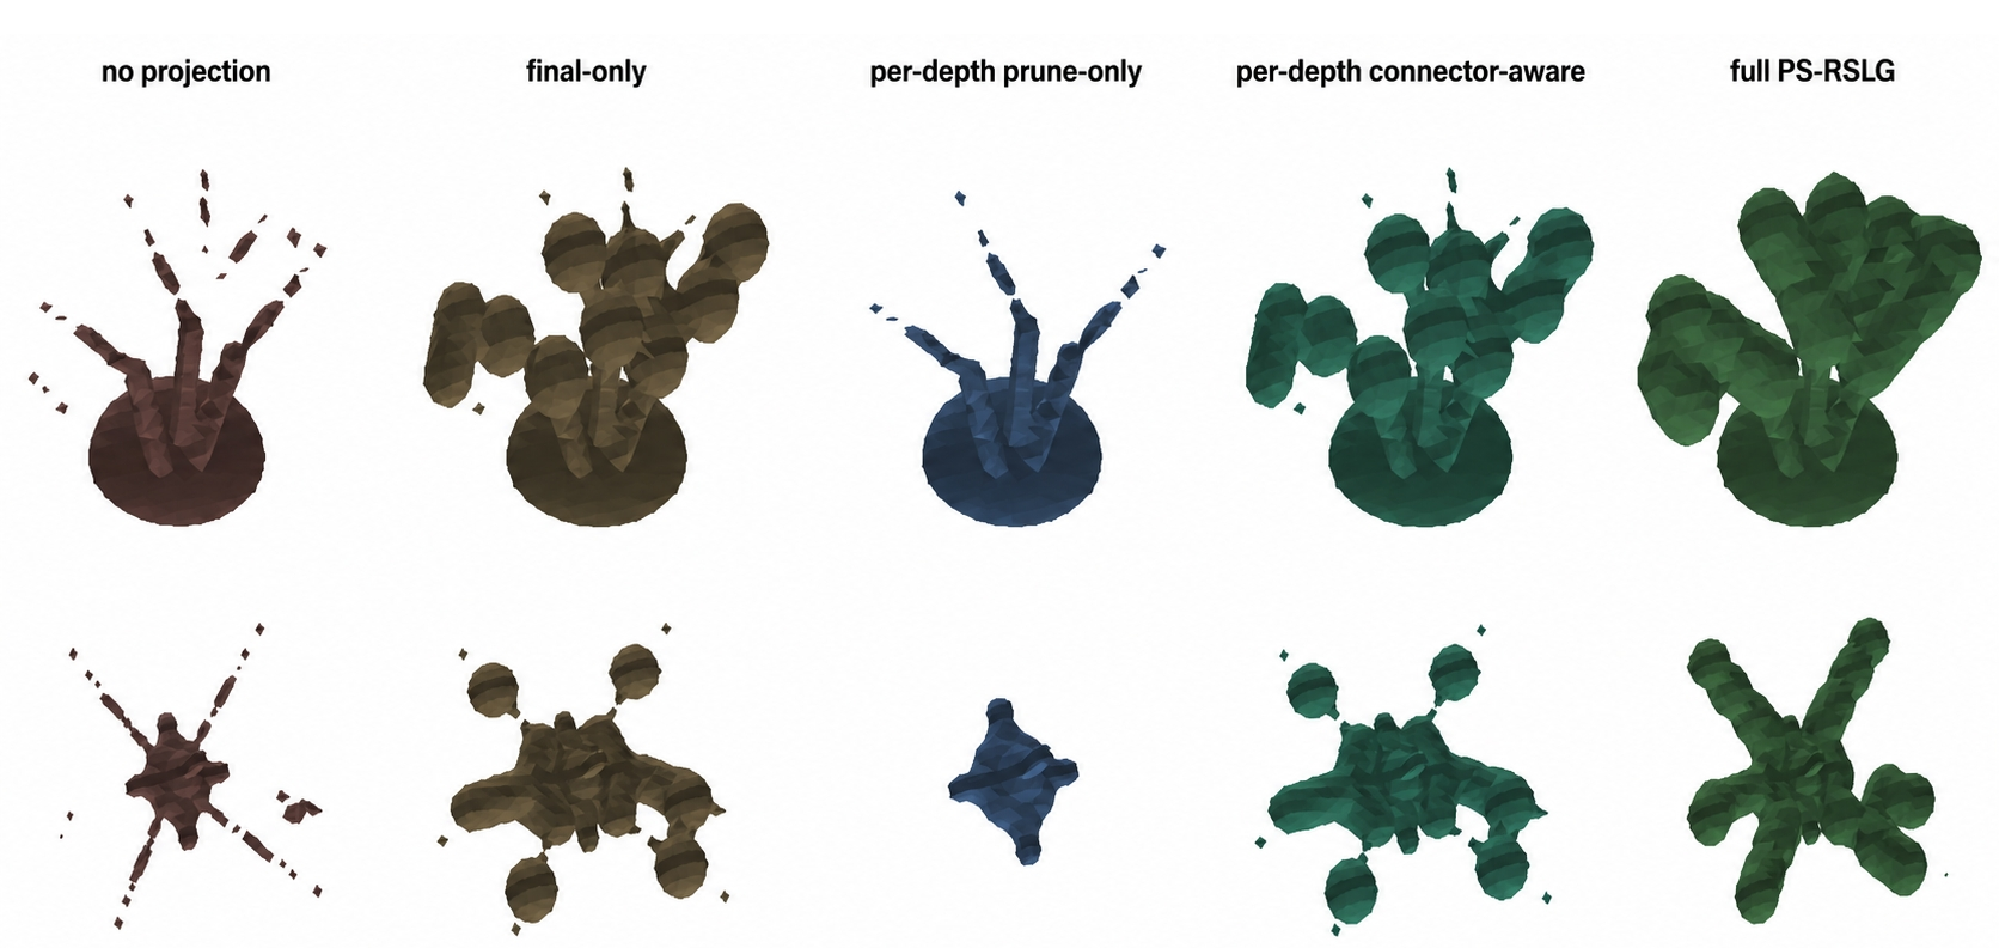
\includegraphics[width=0.92\textwidth]{figures/personal/projection_ablation.pdf}
  \Description{PPTX-composed white-background projection ablation with two visual cases, coral frontier and IFS crystal, comparing no projection, final-only projection, per-depth prune-only projection, per-depth connector-aware projection, and our row with overview and independent zoom rows.}
  \caption{Projection ablation visual companion comparing terminal cleanup with per-depth projected recursive state updates.}
  \label{fig:projection-ablation-mesh}
\end{figure}

\begin{figure}[!htbp]
  \centering
  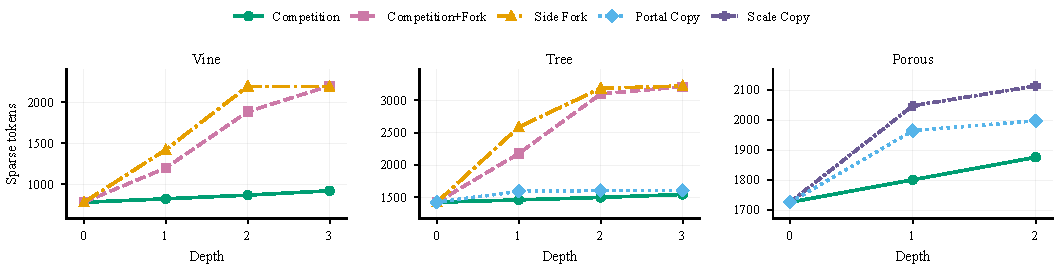
\includegraphics[width=0.88\textwidth]{figures/space_competition_depth_curves_tokens_20260508.pdf}
  \Description{Sparse-token growth curves comparing conservative competition, fork, side-branch, portal, and scale-down recursive operators.}
  \caption{Sparse-token growth curves for recursive operators under matched depth schedules.}
  \label{fig:space-competition-depth-curves}
\end{figure}

\clearpage

\begin{figure}[!htbp]
  \centering
  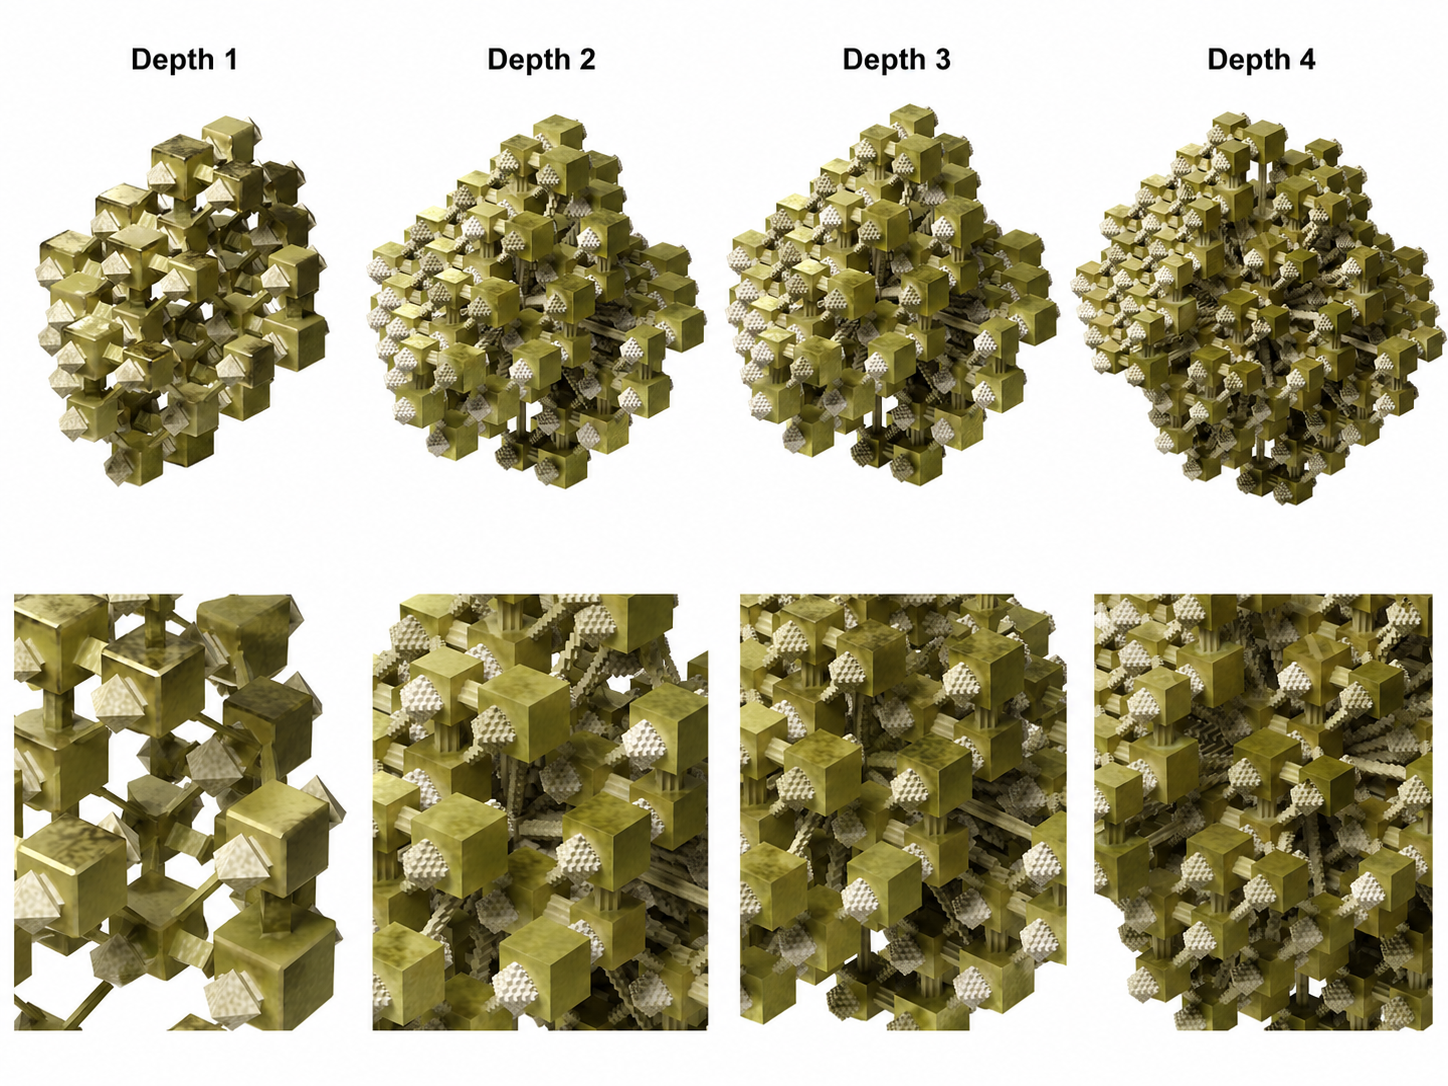
\includegraphics[width=0.78\textwidth]{figures/personal/huangtong.png}
  \Description{Depth-control showcase for a pyrite-like lattice scaffold with faceted rendered surfaces.}
  \caption{Depth control on a connected pyrite-like lattice scaffold under a fixed rendering protocol.}
  \label{fig:pyrite-hq-depth-textured}
\end{figure}

\begin{figure}[!htbp]
  \centering
  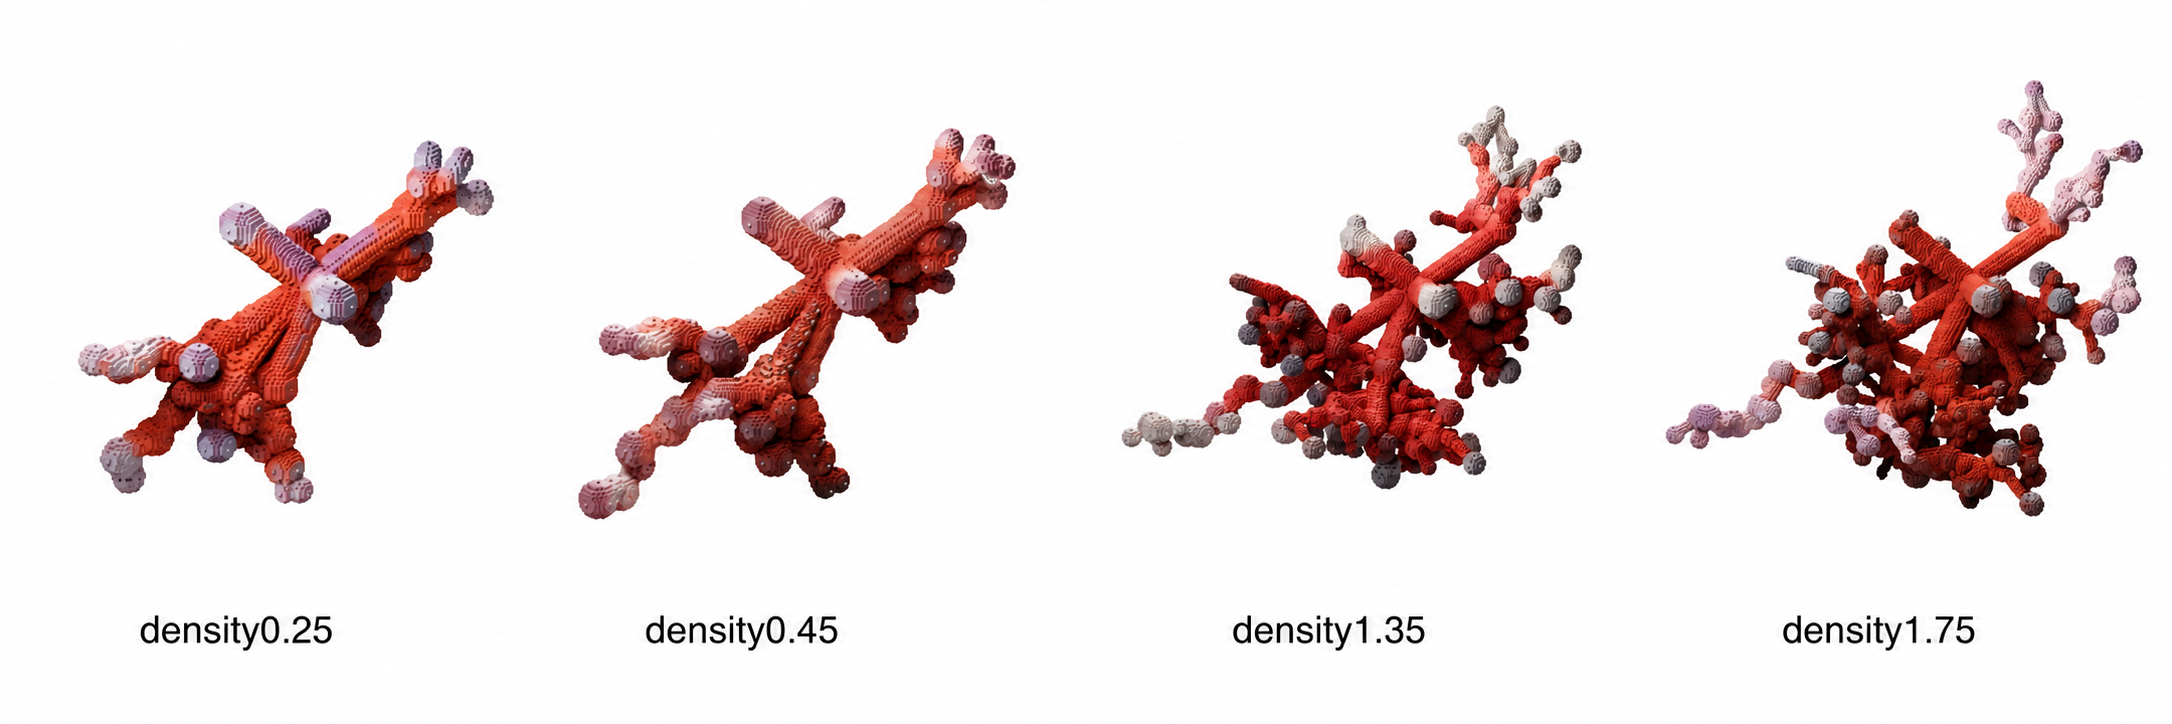
\includegraphics[width=0.92\textwidth]{figures/personal/density_control.png}
  \Description{Same-condition density-parameter control for a connected coral scaffold, showing several density settings.}
  \caption{Density control for a connected coral scaffold under a fixed root descriptor and rule family.}
  \label{fig:coral-density-extreme}
\end{figure}


\clearpage
\twocolumn
\appendix

\section{Operational Projection Routine}
\label{app:projection-routine}
Algorithm~\ref{alg:admissibility-projection} specifies the projection operation used in Sec.~\ref{sec:projection-ablation}. It operates on the decoded candidate, updates the root descriptor and handle registry, and returns the decoded projected asset consumed by codec re-entry in Algorithm~\ref{alg:ps-rsle-execution}.

\begin{algorithm}[t]
  \caption{State-stabilizing admissibility projection.}
  \label{alg:admissibility-projection}
  \begin{algorithmic}[1]
    \Require decoded candidate $x_{d+1}$, candidate handles $\widetilde A_{d+1}$, previous state $s_d$, certificates $\Gamma_d$, thresholds $\lambda_d$
    \Ensure projected asset $x^\star_{d+1}$, root descriptor $r_{d+1}$, projected decoded handle registry $\widehat A_{d+1}$, and codec correspondence $\kappa_{d+1}$
    \State Sample or voxelize $x_{d+1}$ to obtain projection support $U$.
    \State Instantiate root seeds $U^{\mathrm{root}}\subseteq U$ from the persistent root descriptor in $s_d$.
    \State Build the neighborhood graph $G_\eta(U)$.
    \State Compute root-attached support $U^{\mathrm{att}}$ reachable from $U^{\mathrm{root}}$.
    \State Form projected support from $U^{\mathrm{att}}$ and rule-certified connectors satisfying $\Gamma_d$ and $\lambda_d$.
    \For{each handle $h_i\in \widetilde A_{d+1}$}
      \State Locate the owned or target support of $h_i$ by declared proposal transform, overlap, or codec correspondence.
      \If{$h_i$ is root-attached or connector-certified, and all handle constraints remain valid}
        \State Keep $h_i$ active and update its support and frame metadata.
      \Else
        \State Deactivate $h_i$ and exclude it from $A_{d+1}^{\mathrm{act}}$.
      \EndIf
    \EndFor
    \State Construct $x^\star_{d+1}$ from the projected support and surviving decoded geometry.
    \State Update the root descriptor to $r_{d+1}$ from projected root seeds and support.
    \State \Return $x^\star_{d+1}$, $r_{d+1}$, projected decoded handle registry $\widehat A_{d+1}$, and codec correspondence $\kappa_{d+1}$.
  \end{algorithmic}
\end{algorithm}



\section{Additional Tables}
\label{app:moved-main-tables}
The following tables provide compact implementation and evaluation detail for the focused main-paper evidence.

\begin{table*}[t]
  \centering
  \caption{Rule families used to instantiate the proposal interface. Each family reads active handles, emits proposal records, and supports one or more recursive asset structures.}
  \label{tab:rule-families}
  \begin{tabular}{@{}p{0.16\textwidth}p{0.24\textwidth}p{0.34\textwidth}p{0.20\textwidth}@{}}
    \toprule
    Rule family & Reads from active state & Proposal record & Supported structures \\
    \midrule
    \textbf{Branch / grow} &
    Tip, branch, or frontier handles &
    Local support seeds, child handles, parent--child attachment metadata, and editable control regions. &
    Roots, vines, tree crowns, fern-like forms. \\
    \textbf{Frontier attach / accrete} &
    Active frontier handles &
    Stochastic or attraction-guided support seeds with attachment and frontier-update metadata. &
    Coral-like growth, porous aggregates, accretive clusters. \\
    \textbf{Transform-copy} &
    Motif, frame, or reusable-part handles &
    Transformed support seeds, copied feature seeds, candidate motif handles, and transform metadata. &
    Crystals, lattices, repeated motifs. \\
    \textbf{Split / extrude} &
    Frame, tile, portal, or segment handles &
    Bounded extrusion or repetition support with child frame handles and local metadata. &
    Interface-supported hard-surface motifs. \\
    \bottomrule
  \end{tabular}
\end{table*}

\begin{table*}[t]
  \centering
  \caption{Coverage matrix connecting classical recursive systems to executor rule families, exemplar tasks, matched controls, and one-to-one evaluation metrics.}
  \label{tab:coverage-exemplar-tasks}
  \begin{tabular}{@{}p{0.15\textwidth}p{0.20\textwidth}p{0.23\textwidth}p{0.21\textwidth}p{0.13\textwidth}@{}}
    \toprule
    Classical family & Controls & Executor operator family & Exemplar tasks & Primary metrics \\
    \midrule
    L-system & depth, angle, scale decay, branch probability & Branch handles with local frames and attachment certificates & pine branch, root fork, vine split & root reachability, handle survival, surface LCR \\
    Space colonization & attractors, kill radius, influence radius, tip budget & Grow rules with occupancy competition and attractor fields & tree canopy, root network, bush & surface LCR, welded components, handle survival \\
    DLA/frontier & frontier mask, stickiness, random seed, particle budget & Attach rules plus connector masks and projection & coral cluster, porous mineral, accretive root & occupancy components, orphan handles, valid execution \\
    IFS/fractal & transform set, contraction, depth, orbit schedule & Transform-copy rules with masked merge and projection & lattice motif, portal ring, fractal ornament & occupancy LCR, welded components, reusable motif handles \\
    \bottomrule
  \end{tabular}
\end{table*}


\section{Handle-State Summary}
\label{app:state-proxy-audit}
Table~\ref{tab:projection-admissible-state-proxy-summary} summarizes handle-state behavior over the twelve-row projection and masked-local blocks. It complements the mean aggregation in Table~\ref{tab:projection-ablation} by reporting root reachability, orphan active handles, handle survival, strict pass counts, occupancy--state differences, and connector-survival differences before later rule selection.

\begin{table*}[t]
  \centering
  \small
  \setlength{\tabcolsep}{4pt}
  \caption{Handle-state summary for projection and masked-local variants, reporting strict-pass counts, occupancy--state differences, and connector-survival differences across the twelve-row blocks.}
  \label{tab:projection-admissible-state-proxy-summary}
  \resizebox{\textwidth}{!}{%
  % Derived from results/metric_enrichment_20260513/linnaeus_handle_lineage_audit_20260513.csv
\begin{tabular}{lrrrrrrr}
\toprule
Variant & Rows & Strict pass & Med. root reach. & Med. orphan active & Med. handle surv. & Occ.-state diff. & Conn. surv. diff. \\
\midrule
no projection & 12 & 0 & 0.629 & 2.5 & 0.629 & 0.266 & -0.107 \\
final-only projection & 12 & 0 & 0.629 & 2.5 & 0.629 & 0.370 & -0.107 \\
per-depth prune-only & 12 & 3 & 1.000 & 0.0 & 0.736 & -0.019 & 0.000 \\
per-depth connector-aware & 12 & 9 & 1.000 & 0.0 & 1.000 & -0.001 & 0.264 \\
Ours & 12 & 12 & 1.000 & 0.0 & 1.000 & 0.000 & 0.264 \\
masked local/no projection & 12 & 0 & 0.629 & 2.5 & 0.629 & 0.269 & -0.107 \\
masked local/+projection & 12 & 12 & 1.000 & 0.0 & 1.000 & 0.000 & 0.264 \\
\bottomrule
\end{tabular}

  }
\end{table*}

\section{Additional Mesh Measurements}
\label{app:mesh-diagnostic-audit}
Table~\ref{tab:masked-naturalization-topology-audit} reports CPU mesh-topology measurements for the local-realization manifest subset. The measurements cover 18 meshes, three rows per variant. Raw and welded component counts are medians over each variant. All rows in this subset are watertight under the Trimesh check. Blend, masked, and global local realization reduce the median welded component count to one on this manifest, complementing the projection and handle-survival metrics in the main ablation.

\begin{table*}[t]
  \centering
  \small
  \setlength{\tabcolsep}{4pt}
  \caption{Mesh-topology measurements for the local-realization manifest subset, reporting median raw and welded components plus counted watertight rows.}
  \label{tab:masked-naturalization-topology-audit}
  \resizebox{\textwidth}{!}{%
  % Auto-generated summary from results/metric_enrichment_20260513/masked_naturalization_topology_summary_20260513.csv
\begin{tabular}{lrrrrr}
\toprule
Variant & Raw comp. & Weld comp. & Boundary edges & Nonmanifold edges & Watertight \\
\midrule
rule-only & 16 & 16 & 0 & 0 & 3/3 \\
final-only projection & 4 & 4 & 0 & 0 & 3/3 \\
no-realization/+proj & 4 & 4 & 0 & 0 & 3/3 \\
blend/+proj & 1 & 1 & 0 & 0 & 3/3 \\
masked/+proj & 1 & 1 & 0 & 0 & 3/3 \\
global/+proj & 1 & 1 & 0 & 0 & 3/3 \\
\bottomrule
\end{tabular}

  }
\end{table*}

\section{Classical Procedural Systems as Restricted Rule Families}
\label{app:classical-limits}
Classical procedural systems can be described as restricted executor rule families when learned local realization, projection, sparse generator features, or material-guided rendering are disabled. These reductions define semantic coverage relations between classical rules and the proposed interface.

\paragraph{Iterated function systems.}
An IFS is obtained with one patch handle, transform-copy rules, union merge, identity sampler, and identity projection. For contractions $\{\tau_i\}_{i=1}^k$, the support update is $\mathcal V_{d+1}=\bigcup_i \tau_i(\mathcal V_d)$.

\paragraph{L-systems.}
An L-system is obtained when anchors store a symbol string or turtle-frame graph and rules rewrite synchronously, $w_{d+1}=\prod_{a\in w_d}\rho(a)$. The interpretation operator maps emitted symbols to handles with frame updates and optional branch support.

\paragraph{Space colonization and DLA.}
Space colonization is a grow rule whose proposal direction averages attractor directions assigned to a visible tip. DLA-like accretion is an attach rule that samples exposed frontier cells from a hitting distribution and accepts only attached proposals. In the present paper these families serve as structural baselines for recursive attachment behavior.

\paragraph{Shape grammars and symmetry.}
Shape-grammar and CGA-style programs are typed contextual rules over face, tile, portal, split, extrude, repeat, replace, and transform-copy handles. Symmetry programs can be written by scheduling complete group or lattice orbits, but exact equivariance would require rule selection, merge, masked sampling, projection, codec, and grid quantization to commute with the group action. Accordingly, symmetry is reported as an approximate diagnostic in this paper.

\end{document}
